\documentclass[a4paper,11pt]{article}
%DIF LATEXDIFF DIFFERENCE FILE
%DIF DEL manuscript_part2_2024_hw.tex   Tue Jun 25 09:52:42 2024
%DIF ADD manuscript_part2_2024.tex      Mon Jul  8 15:24:09 2024

\usepackage[margin=2.5cm]{geometry}
\usepackage{booktabs} 
\usepackage{amsmath}
\usepackage{amssymb}
\usepackage{graphicx}
\usepackage{caption}
\usepackage{natbib}
\usepackage{xcolor}
\usepackage{tikz}

\newcommand{\p}{\partial}
\newcommand{\gzm}{{\xi}}%{\gamma z_\text{match}}}
\newcommand{\todo}[1]{\textcolor{red}{$[$#1$]$}}
\newcommand{\RE}{\mathbf{Re}}
\hyphenation{Ol-den-burg}

\DeclareRobustCommand\sampleline[1]{%
  \tikz\draw[#1] (0,0) (0,\the\dimexpr\fontdimen22\textfont2\relax)
  -- (2em,\the\dimexpr\fontdimen22\textfont2\relax);%
}

\providecommand{\keywords}[1]
{
  \small	
  \textbf{\textit{Keywords---}} #1
}

\pdfsuppresswarningpagegroup=1

\author{\DIFdelbegin \DIFdel{hauke-zrick}\DIFdelend \DIFaddbegin \DIFadd{Hauke Wurps and Cedrick Ansorge}\DIFaddend }

\date{Draft \today}
\title{Towards a Universal Veering Profile for Turbulent Ekman Flow at arbitrary Reynolds number - Part 2\\
  \normalsize LES and DNS of Turbulent Ekman Flow \\}
%DIF PREAMBLE EXTENSION ADDED BY LATEXDIFF
%DIF UNDERLINE PREAMBLE %DIF PREAMBLE
\RequirePackage[normalem]{ulem} %DIF PREAMBLE
\RequirePackage{color}\definecolor{RED}{rgb}{1,0,0}\definecolor{BLUE}{rgb}{0,0,1} %DIF PREAMBLE
\providecommand{\DIFadd}[1]{{\protect\color{blue}\uwave{#1}}} %DIF PREAMBLE
\providecommand{\DIFdel}[1]{{\protect\color{red}\sout{#1}}}                      %DIF PREAMBLE
%DIF SAFE PREAMBLE %DIF PREAMBLE
\providecommand{\DIFaddbegin}{} %DIF PREAMBLE
\providecommand{\DIFaddend}{} %DIF PREAMBLE
\providecommand{\DIFdelbegin}{} %DIF PREAMBLE
\providecommand{\DIFdelend}{} %DIF PREAMBLE
\providecommand{\DIFmodbegin}{} %DIF PREAMBLE
\providecommand{\DIFmodend}{} %DIF PREAMBLE
%DIF FLOATSAFE PREAMBLE %DIF PREAMBLE
\providecommand{\DIFaddFL}[1]{\DIFadd{#1}} %DIF PREAMBLE
\providecommand{\DIFdelFL}[1]{\DIFdel{#1}} %DIF PREAMBLE
\providecommand{\DIFaddbeginFL}{} %DIF PREAMBLE
\providecommand{\DIFaddendFL}{} %DIF PREAMBLE
\providecommand{\DIFdelbeginFL}{} %DIF PREAMBLE
\providecommand{\DIFdelendFL}{} %DIF PREAMBLE
%DIF LISTINGS PREAMBLE %DIF PREAMBLE
\RequirePackage{listings} %DIF PREAMBLE
\RequirePackage{color} %DIF PREAMBLE
\lstdefinelanguage{DIFcode}{ %DIF PREAMBLE
%DIF DIFCODE_UNDERLINE %DIF PREAMBLE
  moredelim=[il][\color{red}\sout]{\%DIF\ <\ }, %DIF PREAMBLE
  moredelim=[il][\color{blue}\uwave]{\%DIF\ >\ } %DIF PREAMBLE
} %DIF PREAMBLE
\lstdefinestyle{DIFverbatimstyle}{ %DIF PREAMBLE
	language=DIFcode, %DIF PREAMBLE
	basicstyle=\ttfamily, %DIF PREAMBLE
	columns=fullflexible, %DIF PREAMBLE
	keepspaces=true %DIF PREAMBLE
} %DIF PREAMBLE
\lstnewenvironment{DIFverbatim}{\lstset{style=DIFverbatimstyle}}{} %DIF PREAMBLE
\lstnewenvironment{DIFverbatim*}{\lstset{style=DIFverbatimstyle,showspaces=true}}{} %DIF PREAMBLE
%DIF END PREAMBLE EXTENSION ADDED BY LATEXDIFF

\begin{document} 

\maketitle

\begin{abstract}
  % Introduction % Theoretical profile
  Turbulent Ekman flow is \DIFdelbegin \DIFdel{the simplest }\DIFdelend \DIFaddbegin \DIFadd{a canonical flow }\DIFaddend representation of the atmospheric boundary layer\DIFdelbegin \DIFdel{that exhibits two key properties: the }\DIFdelend \DIFaddbegin \DIFadd{, characterized by a }\DIFaddend logarithmic increase of the wind speed near the surface and a turning of the wind vector aloft. In part I of this work, we derived a formulation of the mean wind velocity profiles of the stationary turbulent Ekman flow based on direct numerical simulation (DNS). Here, we explore the \DIFdelbegin \DIFdel{feasibility of extrapolating }\DIFdelend \DIFaddbegin \DIFadd{extrapolation of }\DIFaddend these profiles to atmospheric Reynolds numbers using large-eddy simulation (LES).
  % Case desription and setup
  We compare theoretical \DIFdelbegin \DIFdel{wind speed profiles of a }\DIFdelend \DIFaddbegin \DIFadd{profiles of the wind vector for }\DIFaddend low Reynolds-number turbulent Ekman flow to results from DNS and LES. This necessitates the inclusion of viscous effects, usually neglected in LES, along with modifications to the standard bottom boundary condition.
  % Results and Discussion
  Analysis of the \DIFdelbegin \DIFdel{grid resolution dependency showed }\DIFdelend \DIFaddbegin \DIFadd{grid-convergence for higher resolution unveils }\DIFaddend a convergence of LES \DIFdelbegin \DIFdel{results }\DIFdelend \DIFaddbegin \DIFadd{data }\DIFaddend towards the theoretical profiles for \DIFdelbegin \DIFdel{low }\DIFdelend \DIFaddbegin \DIFadd{both intermediate }\DIFaddend and high Reynolds numbers. \DIFdelbegin \DIFdel{LES results confirmed that within }\DIFdelend \DIFaddbegin \DIFadd{Our LES thus confirm that--within }\DIFaddend the logarithmic layer (the lowest 10\,\% of the boundary layer)\DIFdelbegin \DIFdel{, }\DIFdelend \DIFaddbegin \DIFadd{--- }\DIFaddend the turning of the wind vector \DIFdelbegin \DIFdel{contributes }\DIFdelend \DIFaddbegin \DIFadd{rotates by }\DIFaddend approximately one-third \DIFdelbegin \DIFdel{to the total rotation }\DIFdelend \DIFaddbegin \DIFadd{of its total rotation across the entirety of the boundary layer}\DIFaddend .
  % Conclusions
  \DIFdelbegin \DIFdel{The notable agreement of the }\DIFdelend \DIFaddbegin \DIFadd{Such agreement of our }\DIFaddend theoretical formulation and LES \DIFdelbegin \DIFdel{results raised }\DIFdelend \DIFaddbegin \DIFadd{data raises }\DIFaddend our confidence in \DIFdelbegin \DIFdel{its reliability for high Reynolds numbers. This }\DIFdelend \DIFaddbegin \DIFadd{the underlying assumptions of the theory and thus }\DIFaddend reinforces the utility of the theoretical profiles as a \DIFdelbegin \DIFdel{true }\DIFdelend reference for intermediate and a quasi-reference for higher Reynolds number simulations.
%


\keywords{Large-Eddy Simulation $\cdot$ Scale separation $\cdot$ Ekman layer $\cdot$ Prandtl layer $\cdot$ Hodograph}
\end{abstract}
%
%%%%%%%%%%%%%%%%%%%%%%%%%%%%%%%%%%%%%%%%%%%%%%%%%%%%%%%%%%%%%%%%%%%%%%%%%%%%%%%%
%
\section{Introduction}

\DIFdelbegin \DIFdel{\todo{start introduction rather with TEF than LES (rather subject than method)}
Large Eddy simulation }\DIFdelend %DIF >  \todo{start introduction rather with TEF than LES (rather subject than method)}
\DIFaddbegin \DIFadd{The interaction of atmospheric boundary layer  (ABL) flow with its lower boundary condition, the surface, is a defining property of the ABL \mbox{%DIFAUXCMD
\citep{stull:1988}}\hspace{0pt}%DIFAUXCMD
. Relevant aspects of the interaction with the boundary not only include its heterogeneity \mbox{%DIFAUXCMD
\citep{avissar:MWR1989,giorgi:RG1997,claussen:BM1991,garratt:BM1990} }\hspace{0pt}%DIFAUXCMD
and roughness \mbox{%DIFAUXCMD
\citep{monin:ARF1970,brutsaert:WRR1975,raupach:AMR1991,kostelecky:JFM2024}}\hspace{0pt}%DIFAUXCMD
, but also a wind veer in favor of the pressure gradient force when the surface is approaced \mbox{%DIFAUXCMD
\citep{ekman:AMA1905}}\hspace{0pt}%DIFAUXCMD
. An important tool with capabilities to model the flow-surface interaction is Large-Eddy Simulation }\DIFaddend (LES)\DIFaddbegin \DIFadd{. Indeed, LES }\DIFaddend is widely used to model turbulent flow in the atmospheric boundary layer (ABL) \citep{stoll2020large}. This includes various applications, such as simulating wind turbine and wind farm wakes, and interactions within wind farm clusters \citep{porte2011large,mehta2014large,breton2017survey}. Furthermore, LES is applied in complex environments like mountainous or urban areas \citep{stoll2020large,garcia2018predictive} and to investigate the dispersion of pollution \cite{han2018large}. These applications typically focus on the lower segment of the ABL on the rotating earth, known as the Prandtl or surface layer. In this layer, the vertical wind speed profile commonly exhibits a logarithmic increase, followed by a prominent change of wind direction within the Ekman layer above. Accurate characterization of how wind speed and direction vary with height is of great importance for wind-power forecasting and projection \citep{optis2014moving}.

The simplest representation of the ABL taking into account rotation \emph{and} the quasi non-turbulent, free atmosphere aloft is the turbulent Ekman flow. It is a horizontally homogeneous, statistically stationary boundary-layer flow over a rotating flat surface. Here we consider the problem under neutral stratification, where the potential temperature is constant across the whole domain. Turbulent Ekman flow shows the key characteristics shaping the real ABL: a logarithmic layer and the Ekman spiral. Near the surface, viscous forces dominate the flow. The stationary ABL-height is then defined by the interplay between turbulent growth due to the shear instability of the configuration \citep{lilly1966instability} and rotational suppression of turbulence due to the Coriolis effect. The system's statistical equilibrium is defined by one single parameter, the Reynolds number $\RE$, signifying the scale separation between the largest and smallest scale within the problem. The largest scales are given by shear-induced eddies constrained by the boundary layer's height, while the smallest scales reside within the dissipative range, where strong viscous forces suppress turbulence. The dimensional mean solution of the turbulent Ekman layer is influenced by three parameters: the geostrophic wind $G$, the Coriolis parameter $f$, and the kinematic viscosity $\nu$. These three parameters define the Reynolds number $Re_D = GD/\nu$. With $D=\sqrt{2\nu/f}$ the Ekman layer depth of a laminar flow we write

\DIFdelbegin \begin{align*}\DIFdel{%DIFDELCMD < \label{red}%%%
 Re_D = \frac{G}{\sqrt{\frac{1}{2}\nu f}}
}\end{align*}%DIFAUXCMD
\DIFdelend \DIFaddbegin \begin{align}\DIFadd{\label{red}
 Re_D = \sqrt{2}\frac{G}{\sqrt{\nu f}}
}\end{align}\DIFaddend 

The mean solutions of the velocity components are functions of only the Reynolds number and the height above the ground $z$: $u(\RE_D,z)$, $v(\RE_D,z)$ (see e.g. \cite{csanady1967resistance}).

Part I of this publication, presents a \DIFdelbegin \DIFdel{theoretical }\DIFdelend framework to predict wind direction and speed across the turbulent Ekman flow, drawing from the works of \cite{csanady1967resistance}, \cite{tennekes1973logarithmic}, and \cite{spalart1989theoretical}. As \cite{spalart1989theoretical}, we use $G$, $f$, and $\nu$ to derive the friction velocity $u_\star$ and the angle $\alpha_\star$ between geostrophic wind and shear stress at the wall. While earlier descriptions of the turbulent Ekman layer were limited to specific parts of the boundary layer, we \DIFdelbegin \DIFdel{give a comprehensive theoretical description of the }\DIFdelend \DIFaddbegin \DIFadd{derive }\DIFaddend mean velocity profiles \DIFdelbegin \DIFdel{that covers the complete ABL and quantifies }\DIFdelend \DIFaddbegin \DIFadd{covering the entire ABL with due regard of changes in }\DIFaddend the Reynolds number. We have shown that the theoretical velocity profiles are in excellent agreement with DNS for \DIFdelbegin \DIFdel{low and intermediate Reynolds number}\DIFdelend \DIFaddbegin \DIFadd{intermediate Reynolds numbers}\DIFaddend . 

However, it remains uncertain, if the extrapolation of the \DIFdelbegin \DIFdel{theory }\DIFdelend \DIFaddbegin \DIFadd{above framework }\DIFaddend towards atmospheric $\RE$ is valid. The substantial separation of scales in the ABL renders direct numerical simulation (DNS) of the entire turbulent flow at scale impossible. Within the framework of LES, only the larger eddies are resolved, that contain the main share of kinetic energy, while turbulent mixing below the subfilter-scale is parameterized. This technique allows for the simulation of the ABL at very high (atmospheric) $\RE$. 

\DIFdelbegin \DIFdel{When using LES in a predictive manner, a common assumption is the accurate reproduction of velocity profiles }\DIFdelend \DIFaddbegin \DIFadd{The accurate representation of mean profiles of velocity}\DIFaddend , i.e. \DIFaddbegin \DIFadd{of }\DIFaddend first-order statistics of the wind field\DIFaddbegin \DIFadd{, is commonly assumed when using LES in a predictive manner  }\DIFaddend \citep{fedorovich2004convective}. Here, we compare LES outcomes to theoretical solutions to determine the validity of this assumption under different conditions. As LES \DIFdelbegin \DIFdel{inherently }\DIFdelend introduces the grid size as an additional \DIFdelbegin \DIFdel{(artificial)parameter}\DIFdelend \DIFaddbegin \DIFadd{parameter (often understood in relation to a filter scale, cf. \mbox{%DIFAUXCMD
\cite{pope2004ten}}\hspace{0pt}%DIFAUXCMD
)}\DIFaddend , we conduct a thorough analysis of its impact on simulation results. \cite{esau2004simulation} and \cite{jiang2018large} have executed similar LES analyses of neutral Ekman layers, however, they introduce an additional parameter by selecting an arbitrary roughness length $z_0$, whereas we derive the parameter $z_0$ corresponding to a fluid with a kinematic viscosity of $\nu = 1.5\cdot10^{-5}$ over flat surface.

Here, we examine three different Reynolds numbers $Re_D$: $1600$, $1.5\cdot10^5$, and $10^6$. While the \DIFdelbegin \DIFdel{low-Re case (}\DIFdelend \DIFaddbegin \DIFadd{case }\DIFaddend $Re_D=1600$ \DIFdelbegin \DIFdel{) }\DIFdelend is also investigated by DNS (cf. part 1 of this study), $Re_D=1.5 \cdot 10^5$ and $10^6$ correspond to the scale separation found in typical atmospheric boundary layers. For \DIFdelbegin \DIFdel{the low-Re case}\DIFdelend \DIFaddbegin \DIFadd{$Re_D=1600$}\DIFaddend , we compare DNS and LES results using the exact same forcing and settings. This is the first comparison of this kind for the turbulent Ekman flow. The LES results converge to the DNS results with decreasing grid cell size. This approach raises our confidence in the LES results to a new level for the direct comparison with a resolving simulation. Furthermore, it allows us to extend the insight from DNS to atmospheric scale where an approach through DNS is clearly infeasible for computational constraints. We observe a clear $\RE$ dependency in the LES results, matching the predictions of the theoretical framework.

The content is structured as follows. Section \ref{universal_profile} provides a complete mathematical description of the turbulent Ekman layer's velocity profiles. A description of the simulated cases and the numerical set-up is given in section \ref{setup}, followed by the presentation of results and its comparison to the theoretical profiles in section \ref{results}. We conclude in section \ref{conclusion}.

\section{A Universal Velocity Profile for the Turbulent Ekman Layer}
\label{universal_profile}

\DIFdelbegin \DIFdel{A universal }\DIFdelend \DIFaddbegin \DIFadd{In this chapter, we introduce the }\DIFaddend velocity profile for the turbulent Ekman layer \DIFdelbegin \DIFdel{is }\DIFdelend developed in part I\DIFdelbegin \DIFdel{of this paper. 
In this chapter, we give a brief mathematical description.
}%DIFDELCMD < 

%DIFDELCMD < %%%
\DIFdelend \DIFaddbegin \DIFadd{. 
}\DIFaddend %Definitions
\DIFdelbegin \DIFdel{The mean velocity profiles for all $\RE$ exhibit a dual scaling nature: in }\DIFdelend \DIFaddbegin \DIFadd{We align the coordinate Ox with the surface stress, Oz points normal to the surface and normal to Ox, and Oy in the span-wise direction, normal to Oxz.
%DIF > The mean velocity profiles for all $\RE$ exhibit a dual scaling nature: in proximity to the lower boundary, the velocity profiles collapse when scaled using
In }\DIFaddend proximity to the lower boundary, the \DIFdelbegin \DIFdel{velocity profiles collapse when scaled using }\DIFdelend \DIFaddbegin \DIFadd{boundary layer scales in }\DIFaddend viscous (inner) units, denoted by the index ``$+$'' ($z^+ = zu_\star/\nu$, $U^+=U/u_\star$, where $U$ is the velocity component in x-direction \DIFaddbegin \DIFadd{and $u_\star = \sqrt{\nu \p_z U}$ the friction velocity}\DIFaddend ). From the top perspective, the profiles converge when scaled using outer units, denoted by the index ``$-$'' ($z^-=z/\delta$, $U^-=U/G$, \DIFdelbegin \DIFdel{with }\DIFdelend \DIFaddbegin \DIFadd{where }\DIFaddend $\delta=u_\star/f$ \DIFdelbegin \DIFdel{representing the boundary layer height). The outer and inner velocities }\DIFdelend \DIFaddbegin \DIFadd{is the boundary-layer depth scale, $f$ the Coriolis parameter and }\DIFaddend $G$ \DIFdelbegin \DIFdel{and $u_\star$, respectively, are linked by a semi-empirical law \mbox{%DIFAUXCMD
\cite{spalart1989theoretical}}\hspace{0pt}%DIFAUXCMD
}\DIFdelend \DIFaddbegin \DIFadd{the geostrophic wind speed)}\DIFaddend . 
At the lower boundary, the x-axis of the inner units aligns with the shear stress, while the x-axis of the outer units aligns with the geostrophic wind. The angle between both axes is denoted \DIFdelbegin \DIFdel{by }\DIFdelend \DIFaddbegin \DIFadd{as }\DIFaddend $\alpha_\star$\DIFdelbegin \DIFdel{.
}\DIFdelend \DIFaddbegin \DIFadd{, the surface veer of the wind across the boundary layer. 
%DIF > 
Profiles of the velocity components are studied in three different layers reflecting the change of dominant balance when moving away from the surface. These are
(i) the Ekman layer denoted $(\cdot)_\text{Ek}$ (Sec.~\ref{sec:ekmanlayer}), 
(ii) the viscous sub-layer, denoted by an index $(\cdot)_\text{visc}$, 
and (iii) the logarithmic layer denoted by $(\cdot)_\text{log}$
We match $U_\text{visc}$ and $U_\text{log}$ according to their respective formulations and combine them to $U_\text{inner}$ (Sec.~\ref{sec:innerlayer}).
Inner and outer profiles are then matched by a weighting transfer function based on the error function. 
%DIF > The span-wise component of the velocity is separated into two layers, namely the inner layer $V_\text{inner}$, and the Ekman layer $V_{EK}$. 
}\DIFaddend 

\DIFdelbegin \subsection{\DIFdel{Drag-Law}}
%DIFAUXCMD
\addtocounter{subsection}{-1}%DIFAUXCMD
\DIFdelend %DIF >  \subsection{Drag-Law}

The geostrophic drag\DIFdelbegin \DIFdel{$Z \equiv u_\star/G$ and }\DIFdelend \DIFaddbegin \DIFadd{, i.e. normalized friction $Z\equiv u_\star/G$, and $\alpha_\star$ form the basis of the boundary-layer scaling, and they are estimated using }\DIFaddend the \DIFdelbegin \DIFdel{angle between the shear stress and the geostrophic wind $\alpha_\star$ are two key parameters of the Ekman flow. They can be estimated using a }\DIFdelend semi-empirical drag-law \DIFdelbegin \DIFdel{based on }\DIFdelend \DIFaddbegin \DIFadd{introduced by }\DIFaddend \cite{spalart1989theoretical}, which describes them as functions of only the Reynolds number:
\begin{subequations}\DIFdelbegin %DIFDELCMD < \label{drag}
%DIFDELCMD < 	%%%
\begin{align*}
		\DIFdel{\frac{G}{u_\star}\cos\phi^\star }&\DIFdel{= \frac{1}{\kappa}\log Re_\tau + C - A_r, }\\
		\DIFdel{\sin\phi^\star }&\DIFdel{= A_i\frac{u_\star}{G},}\\
		\DIFdel{\alpha_\star }&\DIFdel{= \phi^\star - \frac{C_5}{Re_\tau},}\\
		\DIFdel{Re_\tau }&\DIFdel{= \frac{u_\star^2}{\nu f},
	}\end{align*}%DIFAUXCMD
\DIFdelend \DIFaddbegin \label{eqn:drag}
	\begin{align}
		\DIFadd{\frac{G}{u_\star}\cos\phi^\star }&\DIFadd{= \frac{1}{\kappa}\log Re_\tau + C - A_r, }\\
		\DIFadd{\sin\phi^\star }&\DIFadd{= A_i\frac{u_\star}{G},}\\
		\DIFadd{\alpha_\star }&\DIFadd{= \phi^\star - \frac{C_5}{Re_\tau},}\\
		\DIFadd{Re_\tau }&\DIFadd{= \frac{u_\star^2}{\nu f} \left( = \frac{1}{2} Re_{D}^2 \frac{u_{\star}^2}{G^2}\right),
	}\end{align}\DIFaddend 
\end{subequations}
\DIFdelbegin \DIFdel{with $Re_\tau = \frac{Re_D^2}{2}\frac{u_\star^2}{G^2}$ the turbulent Reynolds number, }\DIFdelend \DIFaddbegin \DIFadd{where we use }\DIFaddend $\kappa = 0.416$, $A_r = 4.80$, $A_i = -5.57$, $C = 5.4605$, $C_5 = -57.8$ \DIFdelbegin \DIFdel{. This law is in excellent agreement with DNS in the range $400\leq Re_D\leq 1\,600$ as demonstrated by \mbox{%DIFAUXCMD
\cite{ansorge2014global}}\hspace{0pt}%DIFAUXCMD
}\DIFdelend \DIFaddbegin \DIFadd{based on the DNS data available (cf. Part I, \mbox{%DIFAUXCMD
\cite{ansorge2014global}}\hspace{0pt}%DIFAUXCMD
)}\DIFaddend .

\DIFdelbegin \subsection{\DIFdel{Total profile}}
%DIFAUXCMD
\addtocounter{subsection}{-1}%DIFAUXCMD
%DIFDELCMD < 

%DIFDELCMD < %%%
\DIFdel{As frame of reference we use the coordinate system Oxyz with Ox in the direction of the surface stress, Oz normal to the surface, and Oy in the span-wise direction normal to Oxz. The profile of the stream-wise component of the velocity is seperated into three layers, which are the viscous layer $U_{visc}$, the logarithmic layer $U_{log}$, and the Ekman layer $U_{EK}$. $U_{visc}$ and $U_{log}$ are matched by their formulation and combined to $U_{inner}$. The span-wise component of the velocity is separated into two layers, namely the inner layer $V_{inner}$, and the Ekman layer $V_{EK}$. The smooth transition between consecutive layers is achieved using a transfer function:
}\begin{align*}\DIFdel{%DIFDELCMD < \label{error}%%%
  w_{*} = \frac{1}{2}\left(\textrm{erf}\left[\sigma_T\log\left(\frac{z}{z_{T}}\right)\right]+1\right),
}\end{align*}%DIFAUXCMD
\DIFdel{where $erf$ is the error function, $\sigma_T$ is a transition scale that defines the width of the transition and $z_{T}$ is the height of the transition, where the upper and the lower layer equally contribute to the velocity ($w_{*}(z_{T})=0.5$).
}%DIFDELCMD < 

%DIFDELCMD < \begin{subequations}\label{blend}
%DIFDELCMD <   %%%
\begin{align*}
    \DIFdel{U }&\DIFdel{= (1-w_{outer})U_{inner} + w_{outer}U_{EK},}\\
	  \DIFdel{V }&\DIFdel{= (1-w_{outer})V_{inner} + w_{outer}V_{EK}.
	}\end{align*}%DIFAUXCMD
%DIFDELCMD < \end{subequations}
%DIFDELCMD < 

%DIFDELCMD < %%%
\subsection{\DIFdel{Profiles in Outer Layer}}
%DIFAUXCMD
\addtocounter{subsection}{-1}%DIFAUXCMD
\DIFdelend %DIF >  \subsection{Total profile}


\DIFdelbegin \DIFdel{In the outer layer, }\DIFdelend \DIFaddbegin \subsection{\DIFadd{Ekman layer}}
\label{sec:ekmanlayer}
\DIFadd{The outer layer of the ABL is characterized by a triadic balance between turbulent flux, pressure gradient and the Coriolis; }\DIFaddend the vertical change of the Coriolis force causes a pronounced height dependence of the wind direction resulting in the Ekman spiral \DIFdelbegin \DIFdel{\mbox{%DIFAUXCMD
\cite{ekman1905influence}}\hspace{0pt}%DIFAUXCMD
. While the }\DIFdelend \DIFaddbegin \DIFadd{\mbox{%DIFAUXCMD
\citep{ekman:AMA1905}}\hspace{0pt}%DIFAUXCMD
. The }\DIFaddend classic solution employs Ekman dynamics down to the \DIFdelbegin \DIFdel{surface --- and }\DIFdelend \DIFaddbegin \DIFadd{surface---and }\DIFaddend thus also in the surface layer, where \DIFdelbegin \DIFdel{the pure Ekman dynamics are }\DIFdelend \DIFaddbegin \DIFadd{this is }\DIFaddend a rather poor representation of turbulent mixing\DIFdelbegin \DIFdel{---}\DIFdelend \DIFaddbegin \DIFadd{. Here}\DIFaddend , we model the surface layer by a lower boundary condition for the Ekman spiral \DIFdelbegin \DIFdel{that we determine from DNSdata}\DIFdelend \DIFaddbegin \DIFadd{determined from DNS}\DIFaddend :
\begin{subequations}
  \begin{align}
    U_{EK} &= G + Ae^{-\tilde{z}}\cos\tilde{z},\\
		V_{EK} &= - Ae^{-\tilde{z}}\sin\tilde{z},
  \end{align}
\end{subequations}
where the x-axis is aligned with the geostrophic wind and $A = 8.4u_\star$, $\tilde{z} = (z-z_r)/D_E$, $z_r = 0.12\delta$, and $D_E = 3\delta/4\pi\approx 0.24\delta$. The transition from the logarithmic layer to the Ekman layer is located at \DIFdelbegin \DIFdel{$z^-_T=0.3-120/Re_D$ \todo{in script at 0.28- 2.25*np.sqrt(1./re)} }\DIFdelend \DIFaddbegin \DIFadd{$z^{-}=0.28- 2.25 Re_{D}^{-1/2}$ }\DIFaddend with a transition scale of $\sigma_T=2$ for the stream-wise velocity.

\subsection{\DIFdelbegin \DIFdel{Shear-Aligned Velocity}\DIFdelend \DIFaddbegin \DIFadd{Inner and viscous layers}\DIFaddend }
\DIFaddbegin \label{sec:innerlayer}
\DIFaddend 

In the viscous sublayer, the \DIFdelbegin \DIFdel{span-wise velocity is close to zero and the }\DIFdelend shear-aligned velocity \DIFaddbegin \DIFadd{$U^{\alpha_\star}$ }\DIFaddend is described by the law of the wall \DIFdelbegin \DIFdel{:
}%DIFDELCMD < 

%DIFDELCMD < %%%
\begin{align*}
  \DIFdel{U^{\alpha_\star+} = z^+,
}\end{align*}%DIFAUXCMD
\DIFdelend \DIFaddbegin \DIFadd{$U^{\alpha_\star+} = z^+$ and the span-wise velocity $V^{\alpha_\star}$ is zero by choice of the reference frame 
}\DIFaddend (the index $\alpha_\star$ indicates the alignment with the direction of the shear stress). Around $z^+=5$, the velocity \DIFdelbegin \DIFdel{is beginning }\DIFdelend \DIFaddbegin \DIFadd{begins }\DIFaddend to deviate from \DIFdelbegin \DIFdel{its linear profile }\DIFdelend \DIFaddbegin \DIFadd{linearity, }\DIFaddend and the buffer layer forms the transition \DIFdelbegin \DIFdel{between viscous layer and }\DIFdelend \DIFaddbegin \DIFadd{from the viscous to the  }\DIFaddend logarithmic layer. From the surface up to the buffer layer, the stream-wise velocity is described by
\DIFdelbegin \begin{align*}
  \DIFdel{U_{visc}^{\alpha_\star+} = \frac{z^+}{1+c_1(z^+)^2} + (c_2z^+-a_{match})\frac{1+\tanh[0.2(z^+-22)]}{2}+c_3e^{-c_4(z^+-22)^2}.
}\end{align*}%DIFAUXCMD
\DIFdelend \DIFaddbegin \begin{subequations}
  \begin{align}
    \DIFadd{U_\text{buffer}^{\alpha_\star+} = \frac{z^+}{1+c_1(z^+)^2} + (c_2z^+-a_\text{match})\frac{1+\tanh[0.2(z^+-22)]}{2}+c_3e^{-c_4(z^+-22)^2}.
    \label{eqn:ubuffer}
  }\end{align}\DIFaddend 
With $c_1 = 0.00185$, $c_2 = 0.195$\DIFdelbegin \DIFdel{\todo{adapt $c_2$?}}\DIFdelend , $c_3 = 0.4$, $c_4 = 0.35$. The coefficient $a_{match}=3.5727$ is chosen to match the u-profile in the logarithmic layer above at $z^+=40$\DIFdelbegin \DIFdel{.
}%DIFDELCMD < 

%DIFDELCMD < %%%
\DIFdel{The logarithmic region of the stream-wise velocity is 
}\begin{align*}\DIFdel{%DIFDELCMD < \label{log-law}%%%
  U_{\log}^{\alpha_\star+} = \frac{1}{\kappa}\log z^+ + C,
}\end{align*}%DIFAUXCMD
\DIFdelend \DIFaddbegin \DIFadd{, such that 
}\begin{align}
  \DIFadd{U_\text{inner}^{\alpha_\star+} = \begin{cases}
	  U_\text{buffer}^{\alpha_\star+}, & z^+ \le 40.\\
		\kappa^{-1}\log z^+ + C &   z^+>40.
	\end{cases}
  \label{eqn:log-law}
}\end{align}\DIFaddend 
\DIFaddbegin \end{subequations}
\DIFaddend with the von-Kármán constant $\kappa=0.416$, and $C=5.4605$ \DIFdelbegin \DIFdel{. The lower part of $U^{\alpha_\star+}$ is described by
}\begin{align*}
  \DIFdel{U_{inner}^{\alpha_\star+} = \begin{cases}
	  U_{visc}^{\alpha_\star+}, & z^+<40.\\
		U_{log}^{\alpha_\star+}, & z^+>40.
	\end{cases}
}\end{align*}%DIFAUXCMD
%DIFDELCMD < 

%DIFDELCMD < %%%
\DIFdel{The inner profile is then blended to the Ekman profile using eq. \ref{blend} with $\sigma_T = 2$ and $z_T^- = 0.28- 2.25\sqrt{1/Re_D}$. }%DIFDELCMD < 

%DIFDELCMD < %%%
\subsection{\DIFdel{Span-wise Velocity}}
%DIFAUXCMD
\addtocounter{subsection}{-1}%DIFAUXCMD
\DIFdelend \DIFaddbegin \DIFadd{as in the estimation of the geostrophic drag in Eq.~(\ref{eqn:drag}). 
}\DIFaddend 

\DIFdelbegin \DIFdel{In }\DIFdelend \DIFaddbegin \DIFadd{For the span-wise velocity, the boundary conditions and Ekman dynamics imply that 
}\begin{subequations}
\begin{align}
\DIFadd{V^{\alpha_\star}_\text{visc} \delta^+\sim G f_V(z^+),
}\end{align} \DIFadd{where $f_V$ is a universal, non-dimensional function (cf. Part I). Above }\DIFaddend the viscous 
layer, \DIFdelbegin \DIFdel{the shear-aligned }\DIFdelend \DIFaddbegin \DIFadd{scaling arguments are scarce, but there is evidence for a logarithmic scaling of also the 
}\DIFaddend span-wise velocity \DIFdelbegin \DIFdel{is described as
}\begin{align*}
  \DIFdel{V^{\alpha_\star}_{visc} = \frac{G}{\delta^+}v_{ref}(w_vz^+-1+exp}[\DIFdel{-w_vz^+}]\DIFdel{).
}\end{align*}%DIFAUXCMD
\DIFdelend \DIFaddbegin \DIFadd{component. We  hence use  
}\begin{align}
  \DIFadd{V^{\alpha_\star}_\text{inner} = \left\{ \begin{matrix}
      V^{\alpha_\star}_\text{visc} &=& \dfrac{G}{\delta^+}v_{ref}(w_vz^+-1+exp[-w_vz^+])  & z^+ \le 10\\ 
      V_\text{log}^{\alpha_\star}        &=& \dfrac{G}{\delta^+}(a_{log} + b_{log}\log(z^+) + c_{log}z^+) & z^+>10. 
  \end{matrix}\right.
}\end{align}\DIFaddend 
\DIFdelbegin \DIFdel{The choice of $v_{ref} = 18.85$ }\DIFdelend \DIFaddbegin \end{subequations}
\DIFadd{with $v_\text{ref} = 18.85$ }\DIFaddend and $w_v = 0.2353$ leads to excellent agreement with the DNS data. \DIFdelbegin %DIFDELCMD < 

%DIFDELCMD < %%%
\DIFdel{Above the viscous layer a log-like transition to the Ekman layer is modeled by }\begin{align*}
  \DIFdel{V_{log}^{\alpha_\star} = \frac{G}{\delta^+}(a_{log} + b_{log}\log(z^+) + c_{log}z^+).
}\end{align*}%DIFAUXCMD
\DIFdel{A }\DIFdelend \DIFaddbegin \DIFadd{The coefficients $a_\text{log}, b_\text{log}$, and $c_\text{log}$ are determined by (i)-(ii) a }\DIFaddend smooth transition to \DIFdelbegin \DIFdel{$V_{visc}$ }\DIFdelend \DIFaddbegin \DIFadd{$V_\text{visc}$ }\DIFaddend at $z^+=10$\DIFdelbegin \DIFdel{and }\DIFdelend \DIFaddbegin \DIFadd{, and (iii) the condition $V_\text{log}(z^-=0.3) = V_\text{EK}(z^-=0.3) =: v_{03}$ (cf. Part I). For the Reynolds-number dependency of }\DIFaddend the \DIFdelbegin \DIFdel{condition $V_{log}(z^-=0.3) = V_{EK}(z^-=0.3) =: v_{03}$ lead to
}\begin{align*}
  \DIFdel{c_{log} }&\DIFdel{= \frac{v_{03}-v_{10} - d_{10}z_{10}\log(z_{03}/z_{10})}{z_{03}-z_{10}},}\\
	\DIFdel{a_{log} }&\DIFdel{= v_{10}-d_{10}z_{10}\log z_{10}+c_{log}z_{10}(1-\log z_{10}),}\\
	\DIFdel{b_{log} }&\DIFdel{= (d_{10}-c_{log})z_{10}.
}\end{align*}%DIFAUXCMD
\DIFdelend \DIFaddbegin \DIFadd{Ekman-layer profiles, $V_\text{Ek}(z^-=0.3)$ depends on $Re$, such that the coefficients exhibit a weak dependence on $Re$. 
}

\subsection{\DIFadd{Transition from inner to outer profiles, synopsis}}

\DIFadd{A smooth transition between consecutive layers is achieved using a transfer function:
}\begin{align}\DIFadd{\label{eqn:error}
  w_{*} = \frac{1}{2}\left(\textrm{erf}\left[\sigma_T\log\left(\frac{z}{z_{T}}\right)\right]+1\right),
}\end{align}\DIFaddend 
\DIFdelbegin \DIFdel{Here, $d_{10}=4.01$, $v_{10}=27.3$. Because of the $\RE$ dependence of $V_{Ek}$, $v_{03}$ also depends on $\RE$. 
$V_{log}^{\alpha_\star}$ is blended into $V_{EK}$ }\DIFdelend \DIFaddbegin \DIFadd{where $erf$ is the error function, $\sigma_T$ is a transition scale that defines the width of the transition and $z_{T}$ is the height of the transition, where the upper and the lower layer equally contribute to the velocity ($w_{*}(z_{T})=0.5$). The inner profiles $U_\text{inner}$ and $V_\text{inner}$ are blended to the Ekman profile }\DIFaddend using eq.\DIFdelbegin \DIFdel{\ref{blend} }\DIFdelend \DIFaddbegin \DIFadd{~(\ref{eqn:blend}) }\DIFaddend with $\sigma_T = 2$ and $z_T^- = 0.28- 2.25\sqrt{1/Re_D}$.

\DIFdelbegin \subsection{\DIFdel{Profile}}
%DIFAUXCMD
\addtocounter{subsection}{-1}%DIFAUXCMD
\DIFdelend \DIFaddbegin \begin{subequations}\label{eqn:blend}
  \begin{align}
    \DIFadd{U }&\DIFadd{= (1-w_{outer})U_{inner} + w_{outer}U_{EK},}\\
	  \DIFadd{V }&\DIFadd{= (1-w_{outer})V_{inner} + w_{outer}V_{EK}.
	}\end{align}
\end{subequations}
\DIFaddend 

\begin{figure}
  \centerline{
	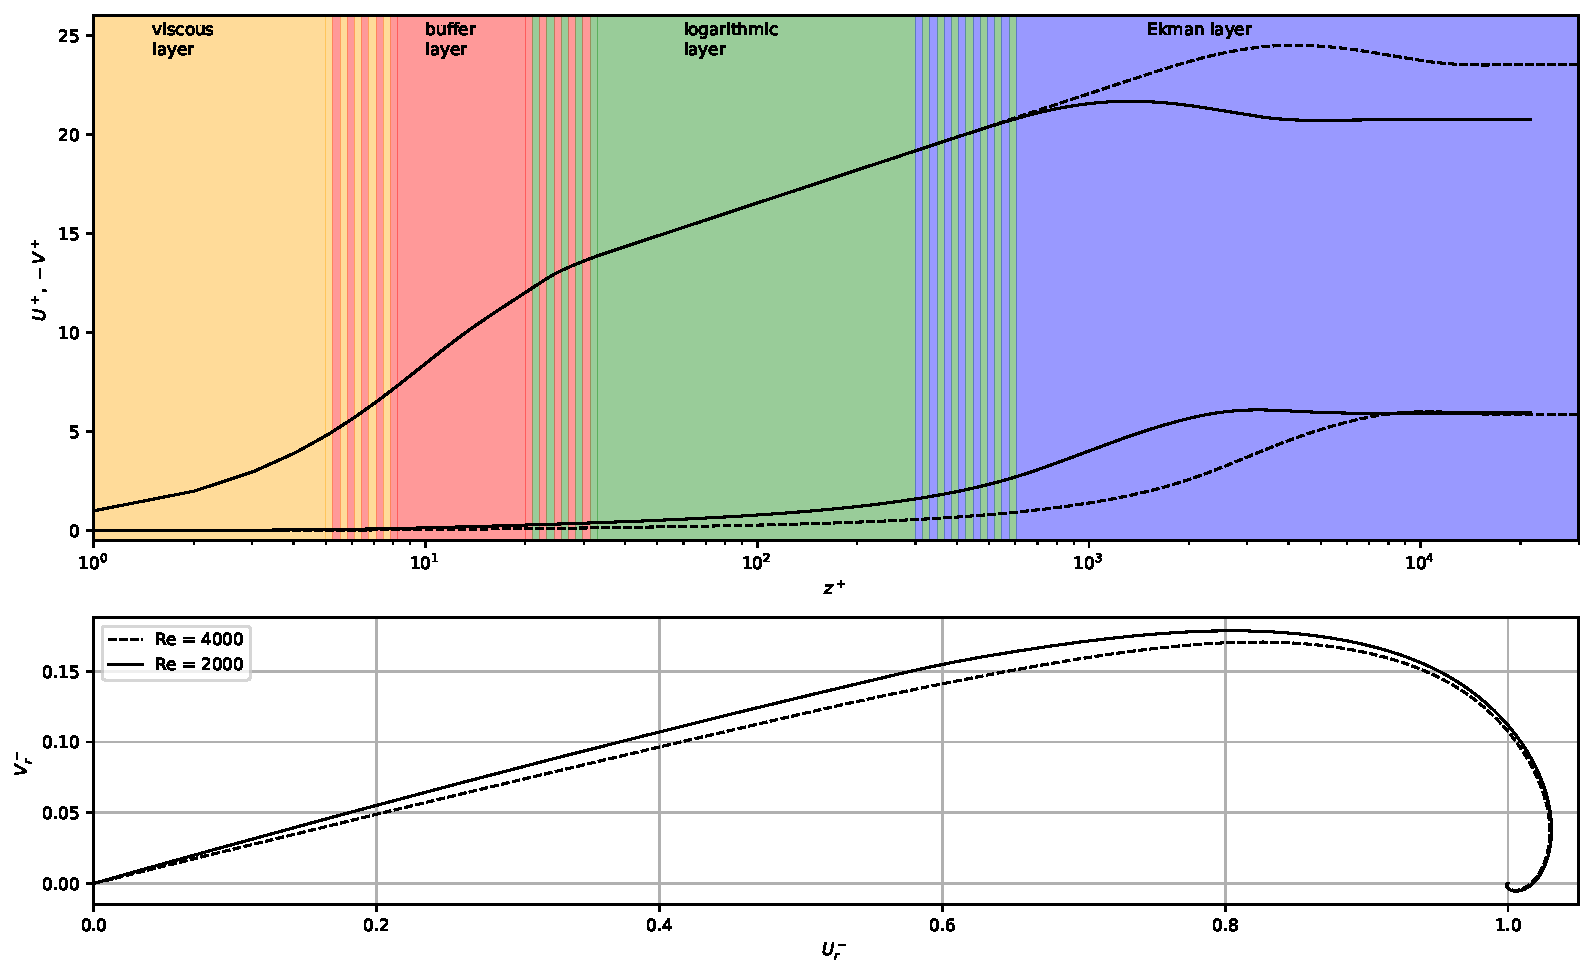
\includegraphics[width=\textwidth]{figures_2024/alt_single_theor_Ekman_profiles_2022.pdf}}
  \caption{a) Theoretical shear-aligned velocity profile ($U^+$,$-V^+$) of the turbulent Ekman flow for $Re_D = 2000$ (\sampleline{}) and $Re_D = 4000$ (\sampleline{dashed}) and the different layers (colors). b) Hodograph of the geostrophy-aligned velocity components}
  \label{single_ekman}. 
\end{figure}

The velocity profiles are given for two Reynolds numbers in Fig. \ref{single_ekman}. 
In the viscous sublayer, the shear-aligned component $U^+$ increases linearly with height up 
\DIFdelbegin \DIFdel{to }\DIFdelend \DIFaddbegin \DIFadd{$z^+\approx5$. In between $5 \lesssim z^+ \lesssim 30$, we find }\DIFaddend the buffer layer \DIFdelbegin \DIFdel{between $z^+\approx5$ and }\DIFdelend \DIFaddbegin \DIFadd{with a transition from the linear law-of-the-wall to the logarithmic law. Above }\DIFaddend $z^+\approx30$, \DIFdelbegin \DIFdel{where it transitions into }\DIFdelend the logarithmic layer \DIFaddbegin \DIFadd{begins}\DIFaddend . Then, $U^+$ increases logarithmically up to the Ekman layer and reaches its supergeostrophic maximum. Above, it decreases to its \DIFaddbegin \DIFadd{free-stream }\DIFaddend geostrophic value. The \DIFdelbegin \DIFdel{length }\DIFdelend \DIFaddbegin \DIFadd{depth }\DIFaddend of the logarithmic layer increases with $\RE$. The spanwise component $V^+$ remains close to zero up to the middle of the logarithmic layer, where the transition to the Ekman layer takes place ($z^-\approx0.28-2.25\sqrt{1/Re_D}$). The profiles of $V^+$ of all Reynolds numbers have a similar shape but are shifted in $z^+$. The similar $V^+$ and the growth of $U^+$ leads to a smaller angle $\alpha_\star$ between surface shear stress and geostrophic wind for higher $\RE$, which is visible in the hodograph.

\section{Case description and numerical set-up}
\label{setup}
%
%\subsection{Notation}
%
%\begin{table*}
	%\centering
%%	\caption{}
	%\begin{tabular}{ll}
    %\toprule
		%$\Delta$ & grid cell size in LES \\
		%$\overline{u''w''}_0$ &  \\
		%$\overline{v''w''}_0$ &  \\
		%$\delta_{95}$ & height where the turbulent stress decreases to 5\% of its surface value\\
		%\bottomrule
	%\end{tabular}
%\end{table*}

\subsection{Settings}

\DIFdelbegin \DIFdel{An incompressible, turbulent Ekman flow over a hydrodynamically smooth surface is simulated for three different Reynolds numbers $Re_D = 10^3;1.5\times 10^5;10^6$, hereafter $Re1$, $Re2$, and $Re3$, respectively. The input parameters are given in table \ref{simulation_parameters}.
}%DIFDELCMD < 

%DIFDELCMD < %%%
\DIFdelend \begin{table*}
	\centering
	\caption{Parameters of the simulated cases. $f$, $\nu$, and $G$ are input parameters and define the Reynolds numbers $Re_D$ and $Re_\tau$, while $u_\star$, $\alpha_\star$, and $\delta = u_\star/f$ are resulting properties of the flow}
	\begin{tabular}{lcccccccc}
          \toprule  
	  Name & $Re_D$ & $Re_\tau$ & $f$ [s$^{-1}$] & $\nu$ [m$^2$s$^{-1}$] & $G$ [ms$^{-1}$] & $u_\star$ [ms$^{-1}$] & $\alpha_\star$ [$^\circ$]& $\delta$ [m] \\
          \midrule
	  Re1 & $1.6\times10^3$ & $3.0\times10^3$ &  &  & 0.0438 & 0.00211 & 16.8 & 21.1 \\
	  Re2 & $1.5\times10^5$ & $7.3\times10^6$ & $10^{-4}$ & $1.5\times10^{-5}$ & 4.108 & 0.1048 & 8.5 & 1048\\
	  Re3 & $1\times10^6$ & $2.2\times10^8$ &  &  & 27.39 & 0.5785 & 7.0 & 5785 \\
          \bottomrule
	\end{tabular}
	\label{simulation_parameters}
\end{table*}
\DIFdelbegin %DIFDELCMD < 

%DIFDELCMD < %%%
\DIFdelend \DIFaddbegin \DIFadd{An incompressible, turbulent Ekman flow over a hydrodynamically smooth surface is simulated using the Parallel Large Eddy Simulation model (PALM, \mbox{%DIFAUXCMD
\citealp{maronga2020overview}}\hspace{0pt}%DIFAUXCMD
). We study three different Reynolds numbers Re$_D = 10^3;1.5\times 10^5;10^6$, hereafter Re1, Re2, and Re3, respectively (Tab.~\ref{simulation_parameters}).
%DIF > 
}\DIFaddend The domain is rotating around the z-axis with an angular velocity corresponding to the Coriolis parameter $f=10^{-4}s^{-1}$. The stratification of the flow is truly neutral, i.e., the potential temperature is constant \DIFdelbegin \DIFdel{for }\DIFdelend \DIFaddbegin \DIFadd{across }\DIFaddend the whole domain. \DIFdelbegin \DIFdel{Nevertheless, the }\DIFdelend \DIFaddbegin \DIFadd{A constant }\DIFaddend boundary layer height \DIFdelbegin \DIFdel{is not growing infinitely but results from a }\DIFdelend \DIFaddbegin \DIFadd{on the order of $\delta=u_\star/f$ forms due to the }\DIFaddend balance between shear production and rotational suppression of turbulence. At the upper boundary, \DIFdelbegin \DIFdel{sufficiently far aloft of the boundary-layer height}\DIFdelend \DIFaddbegin \DIFadd{the flow is non-turbulent. Hence}\DIFaddend , a no-penetration boundary condition is used \DIFdelbegin \DIFdel{and }\DIFdelend \DIFaddbegin \DIFadd{for the vertical velocity component while }\DIFaddend the horizontal components \DIFdelbegin \DIFdel{of the wind are geostrophic, which is a }\DIFdelend \DIFaddbegin \DIFadd{are prescribed according to geostrophic balance--a }\DIFaddend Dirichlet-type boundary condition. At the bottom, a constant-flux layer is assumed and Monin--Obukhov similarity theory (MOST) is used to calculate the surface momentum fluxes. The Navier-Stokes equations are integrated using a \DIFdelbegin \DIFdel{3rd-order }\DIFdelend \DIFaddbegin \DIFadd{3$^\text{rd}$-order }\DIFaddend low-storage \DIFdelbegin \DIFdel{Runge-Kutta }\DIFdelend \DIFaddbegin \DIFadd{Runge--Kutta }\DIFaddend method. For scalar advection a \DIFdelbegin \DIFdel{5th-order }\DIFdelend \DIFaddbegin \DIFadd{5$^\text{th}$-order }\DIFaddend Wicker--Skamarock scheme is employed. The Poisson equation is solved using a direct fast Fourier transform (FFT). In LES, the turbulent transport on the subgrid scale (SGS) needs to be modeled by \DIFdelbegin \DIFdel{a dedicated model, the SGS }\DIFdelend \DIFaddbegin \DIFadd{an SGS closure }\DIFaddend model. We use two \DIFdelbegin \DIFdel{different SGS models to check whether the subgrid closure significantly influences }\DIFdelend \DIFaddbegin \DIFadd{kinds of SGS closures to assess their impact on }\DIFaddend the LES solution: a 1.5-order closure after \cite{deardorff1980stratocumulus} and a dynamic closure after \cite{heinz2008realizability}. For most of the simulations, the 1.5-order closure is used, since the dynamic closure needs more computational resources, but the simulations with $\Delta^-=200^{-1}$ are repeated using the dynamic closure.  
\DIFdelbegin \DIFdel{A comprehensive description of the LES model is given by \mbox{%DIFAUXCMD
\cite{maronga2020overview}}\hspace{0pt}%DIFAUXCMD
.
}\DIFdelend 

\begin{table*}
	\centering
	\caption{Simulations and grid parameters: ReX stands for one of the Reynolds numbers Re1, Re2, and Re3. $\Delta$ is the grid cell size, $\delta=u_\star/f$ is the boundary layer height, $n_i$ is the number of grid cells in the direction $O_i$, $L_x$ and $L_z$ are the domain sizes in the horizontal and vertical direction, respectively}
	  \begin{tabular}{lccccccc}
          \toprule 
	    Name & $\Delta^-$ & $n_x$ & $n_y$ & $n_z$ & $L_x/\delta$ & $L_z/\delta$  \\ 
          \midrule
  	  ReX\_50 & 1/50 & 144 & 144 & 128 & 2.88 & 5.0 \\
  	  ReX\_100 & 1/100 & 288 & 288 & 216 & 2.88 & 4.5 \\
	    ReX\_150 & 1/150 & 432 & 432 & 288 & 2.88 & 3.7 \\
  	  ReX\_200 & 1/200 & 576 & 576 & 384 & 2.88 & 4.1 \\
  	  ReX\_dyn & 1/200 & 576 & 576 & 384 & 2.88 & 4.1 \\
           \bottomrule
		\end{tabular}
	\label{simulation_parameters2}
\end{table*}

To study the effect of resolution on the simulations, four different grid resolutions are chosen for each Reynolds number case. The grid cell size $\Delta$ is around $\delta/50$, $\delta/100$, $\delta/150$, and $\delta/200$, one coarse, two medium, and one fine resolution, respectively (see table \ref{simulation_parameters2}). In total, 15 simulations are carried out. The grid spacing inside the boundary layer is isotropic up to $z = 1.3\delta$. Aloft, the grid spacing along Oz is stretched by 3\% per grid point until a maximum spacing of $(\Delta z )_\mathrm{max} = 6\Delta x$ is reached. The number of vertical grid points is chosen such that $L_z \ge 3 \delta$. Different domain heights are caused by numerical requirements of the FFT-solver. In the upper third of the domain, Rayleigh damping is active to avoid wave reflections from the top boundary.

The flow is initialized with wind speed profiles based on a one-dimensional model with a Reynolds-average based turbulence parametrization. At the beginning of the simulation, random perturbations are imposed on the velocity field to trigger turbulence. The resulting imbalance between pressure force and Coriolis force results in an inertial oscillation of the period $T_{io}=2\pi/f$, where a part of the flow's mean kinetic energy oscillates between U- and V-component. The oscillation decays over time and would eventually vanish for large time. In order to obtain profiles in statistical equilibrium of the flow, we use a spin-up time of 1.5 $T_{io}$ and perform a horizontal domain average over 2 $T_{io}$.

In part I of this publication, the DNS of $Re_D\leq1\,600$ is carried out for a horizontal domain size of $(0.54\Lambda_{Ro})^2$ - $(1.08\Lambda_{Ro})^2$, where $\Lambda_{Ro}=G/f$ is the Rossby radius. For these Reynolds numbers, \DIFdelbegin \DIFdel{$u_\star/G$ is around 0.05 so }\DIFdelend \DIFaddbegin \DIFadd{$Z\approx 0.05$, such that }\DIFaddend $L_x \approx 10 \delta$\DIFdelbegin \DIFdel{However, $u_\star/G$ decreases }\DIFdelend \DIFaddbegin \DIFadd{. However, $Z$ decreases logarithmically }\DIFaddend with increasing Reynolds number and \DIFdelbegin \DIFdel{is around 0.02 }\DIFdelend \DIFaddbegin \DIFadd{it is $Z\approx 0.02$ }\DIFaddend for $Re_D=10^6$. A domain size of half the Rossby radius would then extend to $L_x\approx 25\delta$. Such a large domain would imply immense computational \DIFdelbegin \DIFdel{costs}\DIFdelend \DIFaddbegin \DIFadd{cost}\DIFaddend . \cite{spalart2008direct} used a horizontal domain of $L_x = 2\delta$, arguing that this length allows the resolution of the largest outer-layer eddies according to \cite{csanady1967resistance}. During a sensitivity test of the domain size we observed that simulations with domain sizes $L\geq 4\delta$ often tend to accumulate turbulence kinetic energy in the upper half of the the boundary layer. This TKE increases over several inertial oscillations with energy mostly on the scale of the domain size. Such a development was not observed in the DNS. We could successfully avoid such a behaviour by using a domain of size $L \approx 3\delta$ in combination with a shifted periodic boundary condition in y-direction, as described by \cite{munters2016shifted}. Although for the Ekman flow the direction of the mean flow is only aligned with the x-direction of the grid near the surface, a shift of the boundary condition by $L/3$ significantly helped to suppress the accumulation of TKE in the upper half of the boundary layer.

\subsection{Viscosity and roughness length}

In LES, one postulates that a sufficient part of the largest eddies is resolved so as to represent the dominant non-linear effects of turbulent mixing \citep{pope2004ten}. Below these resolved scales, turbulence is modeled as a more or less isotropically acting diffusive agent by a closure model (dynamic, Deardorff, see above). Thus, molecular friction is not considered directly, but only by virtue of a turbulence model linking the resolved and dissipative scales. In their seminal works on the spectral energy transfer in homogeneous isotropic turbulence, \DIFdelbegin \DIFdel{Kolmogorov and Obukhov (\mbox{%DIFAUXCMD
\cite{kolmogorov1941dissipation} }\hspace{0pt}%DIFAUXCMD
,\mbox{%DIFAUXCMD
\cite{obukhov1941distribution} }\hspace{0pt}%DIFAUXCMD
) }\DIFdelend \DIFaddbegin \DIFadd{\mbox{%DIFAUXCMD
\cite{kolmogorov1941dissipation} }\hspace{0pt}%DIFAUXCMD
and \mbox{%DIFAUXCMD
\cite{obukhov1941distribution} }\hspace{0pt}%DIFAUXCMD
}\DIFaddend showed that the energy transfer rate across the spectrum is in fact \DIFdelbegin \DIFdel{a constant }\DIFdelend \DIFaddbegin \DIFadd{constant provided that both dissipation and production terms can be neglected}\DIFaddend . This implies that the transfer rate across the cut-off scale in LES does not depend on the magnitude of the viscous scale, presupposed that (i) the cut-off scale of the LES is well within the inertial range and (ii) the LES turbulence is approximately isotropic and homogeneous at the smallest resolved scales. Consequently, SGS-models of LES do not necessarily require explicit information about the actual viscosity of the fluid or other viscous parameters.

In LES at low $\RE$ or very high resolution the subgrid eddy viscosities may fall far below the molecular viscosity of air. In the context of PALM's Deardorff closure, it is $K_m = c_0 \Delta \sqrt{e}$, where $c_0 = 0.1$ \citep{deardorff1980stratocumulus}, $\Delta$ is the grid size and $e$ is the SGS-TKE, calculated by a prognostic equation. Hence, very low $e$ as well as fine resolution can lead to $K_m<\nu$. When this is the case, $\nu$ cannot be ignored anymore, and we let $K_m = c_0 \Delta \sqrt{e} + \nu$. \DIFdelbegin \DIFdel{The }\DIFdelend \DIFaddbegin \DIFadd{Hence, (absent stratification) the }\DIFaddend governing equation of \DIFdelbegin \DIFdel{the velocity components in PALM reads
}\begin{align*}\DIFdel{\label{gov_palm}
  \frac{\partial u_i}{\partial t} = - \frac{\partial u_i u_j}{\partial x_j} -\epsilon_{ijk}f_ju_k + \epsilon_{i3j} f_3 u_{g,j} - \frac{1}{\rho_0}\frac{\partial\pi^*}{\partial x_i} + \frac{\partial}{\partial x_j}\left( K_m\left(\frac{\partial u_i}{\partial x_j} + \frac{\partial u_j}{\partial x_i} \right)\right)
}\end{align*}%DIFAUXCMD
\DIFdelend \DIFaddbegin \DIFadd{for momentum in our version of PALM is
}\begin{align}\DIFadd{\label{gov_palm}
  \frac{\partial u_i}{\partial t} = - \frac{\partial u_i u_j}{\partial x_j} -\epsilon_{ijk}f_ju_k + \epsilon_{i3j} f_3 u_{g,j} - \frac{1}{\rho_0}\frac{\partial\pi^*}{\partial x_i} + \frac{\partial}{\partial x_j}\left( K_m\left(\frac{\partial u_i}{\partial x_j} + \frac{\partial u_j}{\partial x_i} \right)\right).
}\end{align}\DIFaddend 
\DIFdelbegin \DIFdel{for a neutrally stratified flow. }\DIFdelend In the limit of either \DIFdelbegin \DIFdel{very well resolved simulations or very }\DIFdelend \DIFaddbegin \DIFadd{well-resolved simulations or }\DIFaddend low $\RE$ (or both), $K_m \rightarrow \nu$, so the last term on the right hand side of eq. (\ref{gov_palm}) becomes $\nu\frac{\partial^2u_i}{\partial x_j^2}$, which complies with the Navier-Stokes equations for an incompressible fluid \DIFaddbegin \DIFadd{underlying our reference solution from DNS}\DIFaddend .

\label{low-bound}

In contrast to the interior closure of the LES where the direct effect of $\nu$ is of small relevance compared to the eddy viscosity---at least for high $\RE$---, this is not true for the viscid effects at the bottom boundary\DIFdelbegin \DIFdel{. Here, a }\DIFdelend \DIFaddbegin \DIFadd{:  A }\DIFaddend constant flux layer is \DIFdelbegin \DIFdel{usually assumed below }\DIFdelend \DIFaddbegin \DIFadd{assumed in between }\DIFaddend the first grid point and the \DIFdelbegin \DIFdel{Monin--Obukhov similarity theory is used to compute the friction velocity and the stresses at the first half grid point (where the horizontal velocities are located }\DIFdelend \DIFaddbegin \DIFadd{lowermost half point (}\DIFaddend on the Arakawa-C staggered grid) \DIFdelbegin \DIFdel{:
}\begin{align*}\DIFdel{%DIFDELCMD < \label{most}%%%
  u_\star = \frac{\kappa(U^2+V^2)^{0.5}}{\ln\left(z/z_0\right)},}\\
  \DIFdel{-\overline{u''w''}_0 = \frac{\kappa Uu_\star}{\ln\left(z/z_0\right)}.
}\end{align*}%DIFAUXCMD
\DIFdelend \DIFaddbegin \DIFadd{to estimate friction velocity and surface stresses by MOST: 
}\begin{align}\DIFadd{\label{most}
  u_\star = \frac{\kappa(U^2+V^2)^{0.5}}{\ln\left(z/z_0\right)},}\\
  \DIFadd{-\overline{u''w''}_0 = \frac{\kappa Uu_\star}{\ln\left(z/z_0\right)}, 
}\end{align}\DIFaddend 
\DIFaddbegin \DIFadd{where double dashes refer to the unresolved, i.e. SGS-parameterized, fluctuations. }\DIFaddend In these expressions, viscosity enters indirectly by virtue of the roughness length $z_0$ when considering the law of the wall for a smooth surface:
\begin{align}
  u^+ = \frac{1}{\kappa}\ln(z^+) + C^+ = \frac{1}{\kappa}\ln\left(\frac{z^+}{z_0^+}\right).
\end{align}
\DIFdelbegin \DIFdel{This leads to the expression
}\begin{align*}
	\DIFdel{z_0^+ = z_0\frac{u_\star}{\nu} = \exp\left(-\kappa C^+\right),
}\end{align*}%DIFAUXCMD
\DIFdel{and for an }\DIFdelend %DIF > This leads to the expression
%DIF > \begin{align}
%DIF > 	z_0^+ = z_0\frac{u_\star}{\nu} = \exp\left(-\kappa C^+\right),
%DIF > \end{align}
\DIFaddbegin \DIFadd{For }\DIFaddend aerodynamically smooth flow, \DIFaddbegin \DIFadd{it is }\DIFaddend $z_0^+ = 0.1031$ \DIFdelbegin \DIFdel{(using the same values as in eq.\ref{log-law}). }\DIFdelend \DIFaddbegin \DIFadd{based on Eq.~\ref{eqn:log-law}. (}\DIFaddend This is known to be the minimal roughness length of a turbulent boundary layer\DIFdelbegin \DIFdel{(}\DIFdelend \DIFaddbegin \DIFadd{; }\DIFaddend see e.g. \DIFdelbegin \DIFdel{\mbox{%DIFAUXCMD
\cite{kraus2008grundlagen}}\hspace{0pt}%DIFAUXCMD
).The roughness length in SI-units 
}\DIFdelend \DIFaddbegin \DIFadd{\mbox{%DIFAUXCMD
\citealp{kraus2008grundlagen}}\hspace{0pt}%DIFAUXCMD
.) Hence,
}\DIFaddend \begin{align}
	z_0 = z_0^+\frac{\nu}{u_\star}\approx 0.1\frac{\nu}{u_\star}
\end{align}
\DIFdelbegin \DIFdel{hence }\DIFdelend depends on the viscosity \DIFaddbegin \DIFadd{$\nu$ }\DIFaddend of the fluid\DIFdelbegin \DIFdel{, which means that---given fixed surface properties---the choice of }\DIFdelend \DIFaddbegin \DIFadd{. In other words, given fixed surface properties, a choice for }\DIFaddend $z_0$ implies a particular value for the viscosity $\nu$.

When using MOST for the surface fluxes it is assumed that the height of the first grid point lies inside of the logarithmic layer. Again, the limit of low $\RE$ and high resolution requires adaptations to this boundary condition. In the case of very fine resolution, the first grid point might fall into the buffer layer or even the viscous layer of the flow, so the equations of MOST are no longer adequate to calculate the local stress. To avoid that, we follow the recommendation of \cite{kawai2012wall} \DIFdelbegin \DIFdel{to }\DIFdelend \DIFaddbegin \DIFadd{and }\DIFaddend use the horizontal velocity from a higher layer $z_{sl}$ to compute the mean stress in the constant flux layer. \DIFdelbegin \DIFdel{Furthermore}\DIFdelend \DIFaddbegin \DIFadd{Further}\DIFaddend , we adopt the boundary condition suggested by \cite{maronga2020improved} and use \DIFdelbegin \DIFdel{the }\DIFdelend domain averaged velocities \DIFdelbegin \DIFdel{:
}\begin{align*}\DIFdel{\label{us_mean}
  u_{*,mean} = \frac{\kappa<u_h(z_{sl})>}{\ln(z_{sl}/z_0)},
}\end{align*}%DIFAUXCMD
\DIFdelend \DIFaddbegin \DIFadd{for the estimation $u_\star$:
}\begin{align}\DIFadd{\label{us_mean}
  u_\star \approx u_{*,mean} = \frac{\kappa<u_h(z_{sl})>}{\ln(z_{sl}/z_0)},
}\end{align}\DIFaddend 
where $u_h= \sqrt{u^2+v^2}$ and angle brackets refer to the horizontal average over the entire domain. The mean stress is then used as a boundary condition at the first grid point ($z=z_1$). It is distributed locally to the \DIFaddbegin \DIFadd{unresolved }\DIFaddend stresses in x- and y-direction via
\DIFdelbegin \begin{align*}
  \DIFdel{\overline{u'w'}_0(x,y,z_1) = -u_{*,mean}^2 \frac{u(x,y,z_1)}{\sqrt{<u>^2(z_1)+<v>^2(z_1)}},
}\end{align*}%DIFAUXCMD
\DIFdelend \DIFaddbegin \begin{align}
  \DIFadd{\overline{u''w''}_0(x,y,z_1) = -u_{*,mean}^2 \frac{u(x,y,z_1)}{\sqrt{<u>^2(z_1)+<v>^2(z_1)}},
}\end{align}\DIFaddend 
and accordingly for \DIFdelbegin \DIFdel{$\overline{v'w'}_0$}\DIFdelend \DIFaddbegin \DIFadd{$\overline{v''w''}_0$}\DIFaddend . This way, the domain average of the stress components yield the total stress of eq. \ref{us_mean} (\DIFdelbegin \DIFdel{$u_{*,mean}^2 = \sqrt{<\overline{u'w'}_0>^2+<\overline{v'w'}_0>^2}$). As }\DIFdelend \DIFaddbegin \DIFadd{$u_{*,mean}^2 = \sqrt{<\overline{u''w''}_0>^2+<\overline{v''w''}_0>^2}$). For the }\DIFaddend reference height we use \DIFdelbegin \DIFdel{$z_{sl}^- \approx 0.1$ (depending on the height of the closest grid level ). By using this higher reference height for the boundary condition we solve }\DIFdelend \DIFaddbegin \DIFadd{the grid level closest to $z_{sl}^- \approx 0.1$. This alleviates }\DIFaddend two problems: First, \DIFdelbegin \DIFdel{the reference height is inside of the logarithmic layer, second, we use a velocity from a region where the flow is much }\DIFdelend \DIFaddbegin \DIFadd{$z_{sl}$ is within log-layer. Second, the flow at $z=z_{sl}$ is }\DIFaddend better resolved than \DIFdelbegin \DIFdel{close }\DIFdelend \DIFaddbegin \DIFadd{closer }\DIFaddend to the surface.

\section{Results and Discussion}
\label{results}

In this chapter, we compare the results from the LES to the theoretical bulk parameters (\ref{bulk}) and velocity profiles (\ref{vel_profiles}) and discuss the dynamics of the turbulent flow in LES.

\subsection{\DIFdelbegin \DIFdel{Bulk parameters}\DIFdelend \DIFaddbegin \DIFadd{Geostrophic drag and surface wind veer}\DIFaddend }
\label{bulk}

\begin{table*}
	\centering
	\caption{LES results: $\Delta^+$ is the grid cell size in wall units, $u_\star$ the friction veloctiy, $\alpha_\star$ the angle between geostrophic wind and negative surface shear stress, $\kappa_{LES}$ the Kármán-measure of the logarithmic layer (estimated by linear regression), $C^+$ the intercept (see eq. \DIFdelbeginFL \DIFdelFL{\ref{log-law}}\DIFdelendFL \DIFaddbeginFL \DIFaddFL{\ref{eqn:log-law}}\DIFaddendFL ), and $\delta_{95}$ the height estimated by a linear interpolation of the shear stress reduction to 95\% of its surface value}
		\begin{tabular}{lcccccc}
		  Name & $\Delta^+$ & $u_\star/u_{\star,th}$ & $\alpha_{\star,th}-\alpha_\star$ & $\kappa_{LES}$ & $C^+$ & $\delta_{95}/\delta$ \\
			\hline
Re1\_50	&	59	&	1.021	&	1.5°	&	-	&	-	&	0.71	\\
Re1\_100	&	30	&	1.008	&	1.1°	&	0.52	&	8.3	&	0.66	\\
Re1\_150	&	20	&	1.004	&	1.0°	&	0.48	&	7.0	&	0.64	\\
Re1\_200	&	15	&	1.003	&	0.7°	&	0.46	&	6.5	&	0.62	\\
Re1\_dyn	&	15	&	1.002	&	0.9°	&	0.43	&	5.7	&	0.58	\\
\hline													
Re2\_50	&	$1.5\times10^5$	&	1.008	&	1.1°	&	-	&	-	&	0.77	\\
Re2\_100	&	$7.3\times10^4$	&	1.001	&	0.5°	&	0.53	&	12.2	&	0.66	\\
Re2\_150	&	$4.9\times10^4$	&	1.000	&	0.2°	&	0.47	&	8.9	&	0.60	\\
Re2\_200	&	$3.7\times10^4$	&	1.000	&	0.1°	&	0.44	&	6.8	&	0.59	\\
Re2\_dyn	&	$3.7\times10^4$	&	1.000	&	0.0°	&	0.42	&	5.6	&	0.55	\\
\hline													
Re3\_50	&	$4.5\times10^6$	&	1.007	&	0.7°	&	-	&	-	&	0.76	\\
Re3\_100	&	$2.2\times10^6$	&	1.001	&	0.5°	&	0.53	&	14.3	&	0.65	\\
Re3\_150	&	$1.5\times10^6$	&	1.000	&	0.3°	&	0.47	&	10.3	&	0.60	\\
Re3\_200	&	$1.1\times10^6$	&	1.001	&	0.1°	&	0.44	&	7.7	&	0.59	\\
Re3\_dyn	&	$1.1\times10^6$	&	1.000	&	0.2°	&	0.43	&	6.7	&	0.56	\\
			\hline
		\end{tabular}
	\label{simulation_results}
\end{table*}

% z0
\DIFdelbegin \DIFdel{A key parameter governing the turbulent state of the flow is the geostrophic drag : it puts the surface friction in relation to the geostrophic wind and thus illustrates }\DIFdelend \DIFaddbegin \DIFadd{The geostrophic drag $Z=u_\star/G$ quantifies }\DIFaddend the conversion of mean-flow kinetic energy \DIFdelbegin \DIFdel{to turbulence}\DIFdelend \DIFaddbegin \DIFadd{($G^2$) to turbulence ($u_{\star}^2$)}\DIFaddend . The ratio of $u_{\star}$ resulting from the simulations to the theoretical value $u_{\star,th}$ are shown in \DIFdelbegin \DIFdel{Tbl}\DIFdelend \DIFaddbegin \DIFadd{Tab}\DIFaddend . \ref{simulation_results}. All values are close to one, while the strongest deviations are observed for the simulations with the coarsest resolutions. A slight dependence on the resolution can be observed for Re1, as $u_\star$ steadily approaches $u_{\star,th}$ with increasing resolution. For Re2 and Re3, all but the coarsest resolution nearly exactly match the theoretical value. The choice of $z_0$ and the geostrophic wind $G$ determine the magnitude of $u_\star$ in a non-trivial way. From a top perspective, the horizontal velocity increases from its geostrophic value to the supergeostrophic maximum and then decreases with decreasing height. The horizontal mean velocity at the grid point closest to $z^-=0.1$ is used to calculate $u_\star$ according to \DIFdelbegin \DIFdel{eq.\ref{us_mean}}\DIFdelend \DIFaddbegin \DIFadd{Eq.~(\ref{us_mean})}\DIFaddend . It is remarkable that the choice of $z_0^+=0.1031$ leads to a value of $u_{\star}$ very close to the prediction by semi-empirical considerations (cf. \cite{spalart1989theoretical}).

\begin{figure}[ht]
	\centering
	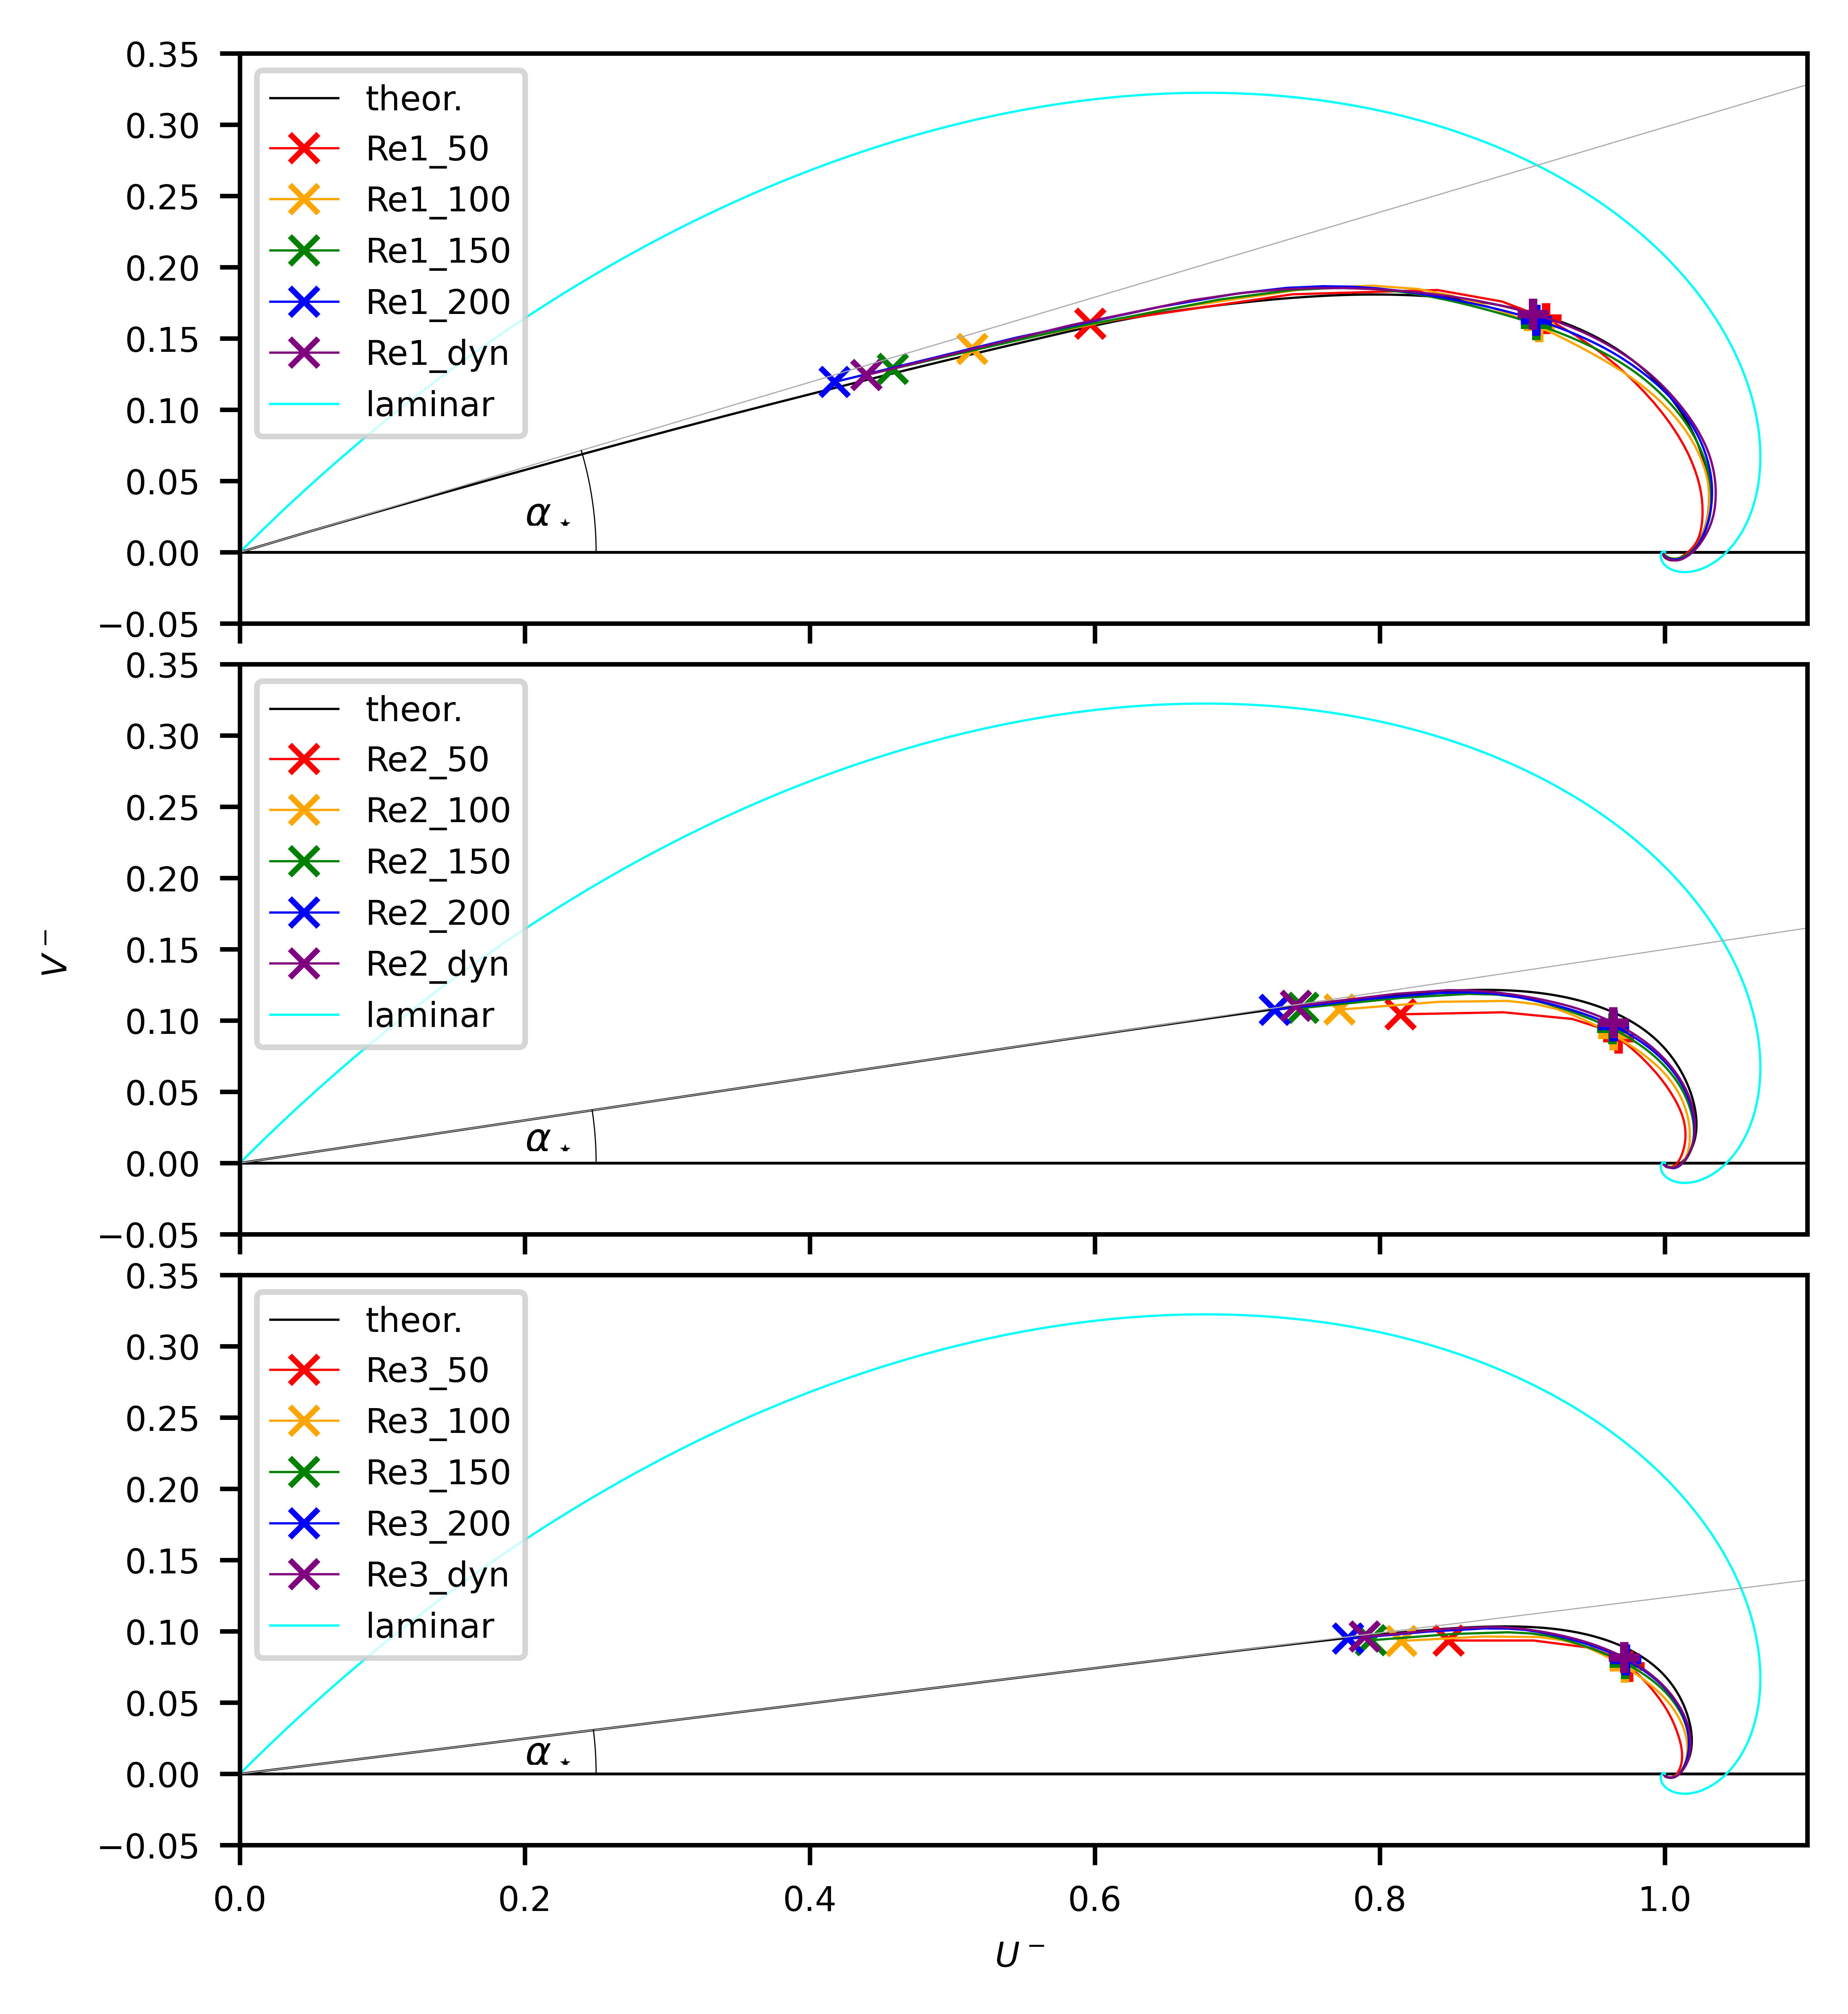
\includegraphics[width=0.7\textwidth]{figures_2024/d3y_3Re_hodograph}
  \caption{Geostrophy aligned hodographs of the LES in comparison to the theoretical and laminar hodographs. A $\times$ indicates the first grid point of the LES. At the points marked with $+$, the velocity is used to determine $u_\star$}
  \label{3Re_hodograph}
\end{figure}

%alpha
\DIFdelbegin \DIFdel{Another key parameter of the Ekman flow is the surface veering angle }\DIFdelend \DIFaddbegin \DIFadd{The surface veering }\DIFaddend $\alpha_\star$ \DIFdelbegin \DIFdel{between the directions of the negative surface shear stress and the geostrophic wind}\DIFdelend \DIFaddbegin \DIFadd{is key to quantify the Ekman pumping and of central relevance for larger-scale applications}\DIFaddend . For the LES, \DIFdelbegin \DIFdel{the direction of the negative stress is represented by }\DIFdelend \DIFaddbegin \DIFadd{we use }\DIFaddend the first derivatives of the velocity components calculated by \DIFdelbegin \DIFdel{3rd order }\DIFdelend \DIFaddbegin \DIFadd{3$^\text{rd}$-order }\DIFaddend forward finite differences \DIFdelbegin \DIFdel{: $\alpha_\star = \tan^{-1}(\langle \partial v/\partial z\rangle_0/\langle \partial u/\partial z\rangle_0)-\tan^{-1}(V_G/U_G)$. Table \ref{simulation_results} shows that nearly }\DIFdelend \DIFaddbegin \DIFadd{to estimate $\alpha_\star$:
}\begin{align}
  \DIFadd{\alpha_\star = \arctan\left(\left.\left\langle \frac{\partial v}{\partial z}\right\rangle_0\right/\left\langle \frac{\partial u}{\partial z}\right\rangle_0\right)-\arctan\left(\frac{V_G}{U_G}\right).
}\end{align}
\DIFadd{Nearly }\DIFaddend all LES yield an $\alpha_\star$ smaller than the theoretical value \DIFdelbegin \DIFdel{$\alpha_{\star,th}$. In general, we observe an }\DIFdelend \DIFaddbegin \DIFadd{$\alpha_{\star,\text{th}}$ (cf. Tab.~\ref{simulation_results}), where we observe a slight }\DIFaddend increase of $\alpha_\star$ with resolution\DIFdelbegin \DIFdel{. }\DIFdelend \DIFaddbegin \DIFadd{; }\DIFaddend The finest resolution of \DIFdelbegin \DIFdel{$Re2$ and $Re3$ }\DIFdelend \DIFaddbegin \DIFadd{Re2 and Re3 }\DIFaddend generally align closely with the theoretical direction while for \DIFdelbegin \DIFdel{$Re1\_200$ still }\DIFdelend \DIFaddbegin \DIFadd{Re1\_200 the offset is }\DIFaddend 0.9°\DIFdelbegin \DIFdel{is missing. Fig}\DIFdelend . \DIFdelbegin \DIFdel{\ref{3Re_hodograph} }\DIFdelend \DIFaddbegin \DIFadd{The hodograph (Fig.~\ref{3Re_hodograph}) }\DIFaddend illustrates that this is not caused by poor quality of the simulation since all of the simulations of \DIFdelbegin \DIFdel{$Re1$ }\DIFdelend \DIFaddbegin \DIFadd{Re1 closely }\DIFaddend follow the theoretical hodograph\DIFdelbegin \DIFdel{quite closely and even overestimate the }\DIFdelend \DIFaddbegin \DIFadd{; in fact, the turning }\DIFaddend angle at the respective height \DIFdelbegin \DIFdel{by a little. In contrast to the higher $\RE$, the }\DIFdelend \DIFaddbegin \DIFadd{is actually slightly overestimated. Rather, the offset is due to the }\DIFaddend veering of the wind vector continues in the lower \DIFdelbegin \DIFdel{parts }\DIFdelend \DIFaddbegin \DIFadd{part }\DIFaddend of the boundary layer \DIFaddbegin \DIFadd{that is not present in the LES}\DIFaddend . Hence, for the low-$\RE$ case, the general observation of a higher $\alpha_\star$ with finer resolution is also caused by the approach of the final $\alpha_\star$ with decreasing height of the first grid point. In general, the finer resolved simulations show veering angles that are very close to the \DIFdelbegin \DIFdel{theoretic predictions}\DIFdelend \DIFaddbegin \DIFadd{theoretical prediction}\DIFaddend .

\subsection{Logarithmic layer stream-wise velocity}
\label{vel_profiles}

\begin{figure}[ht]
  \centerline{
	  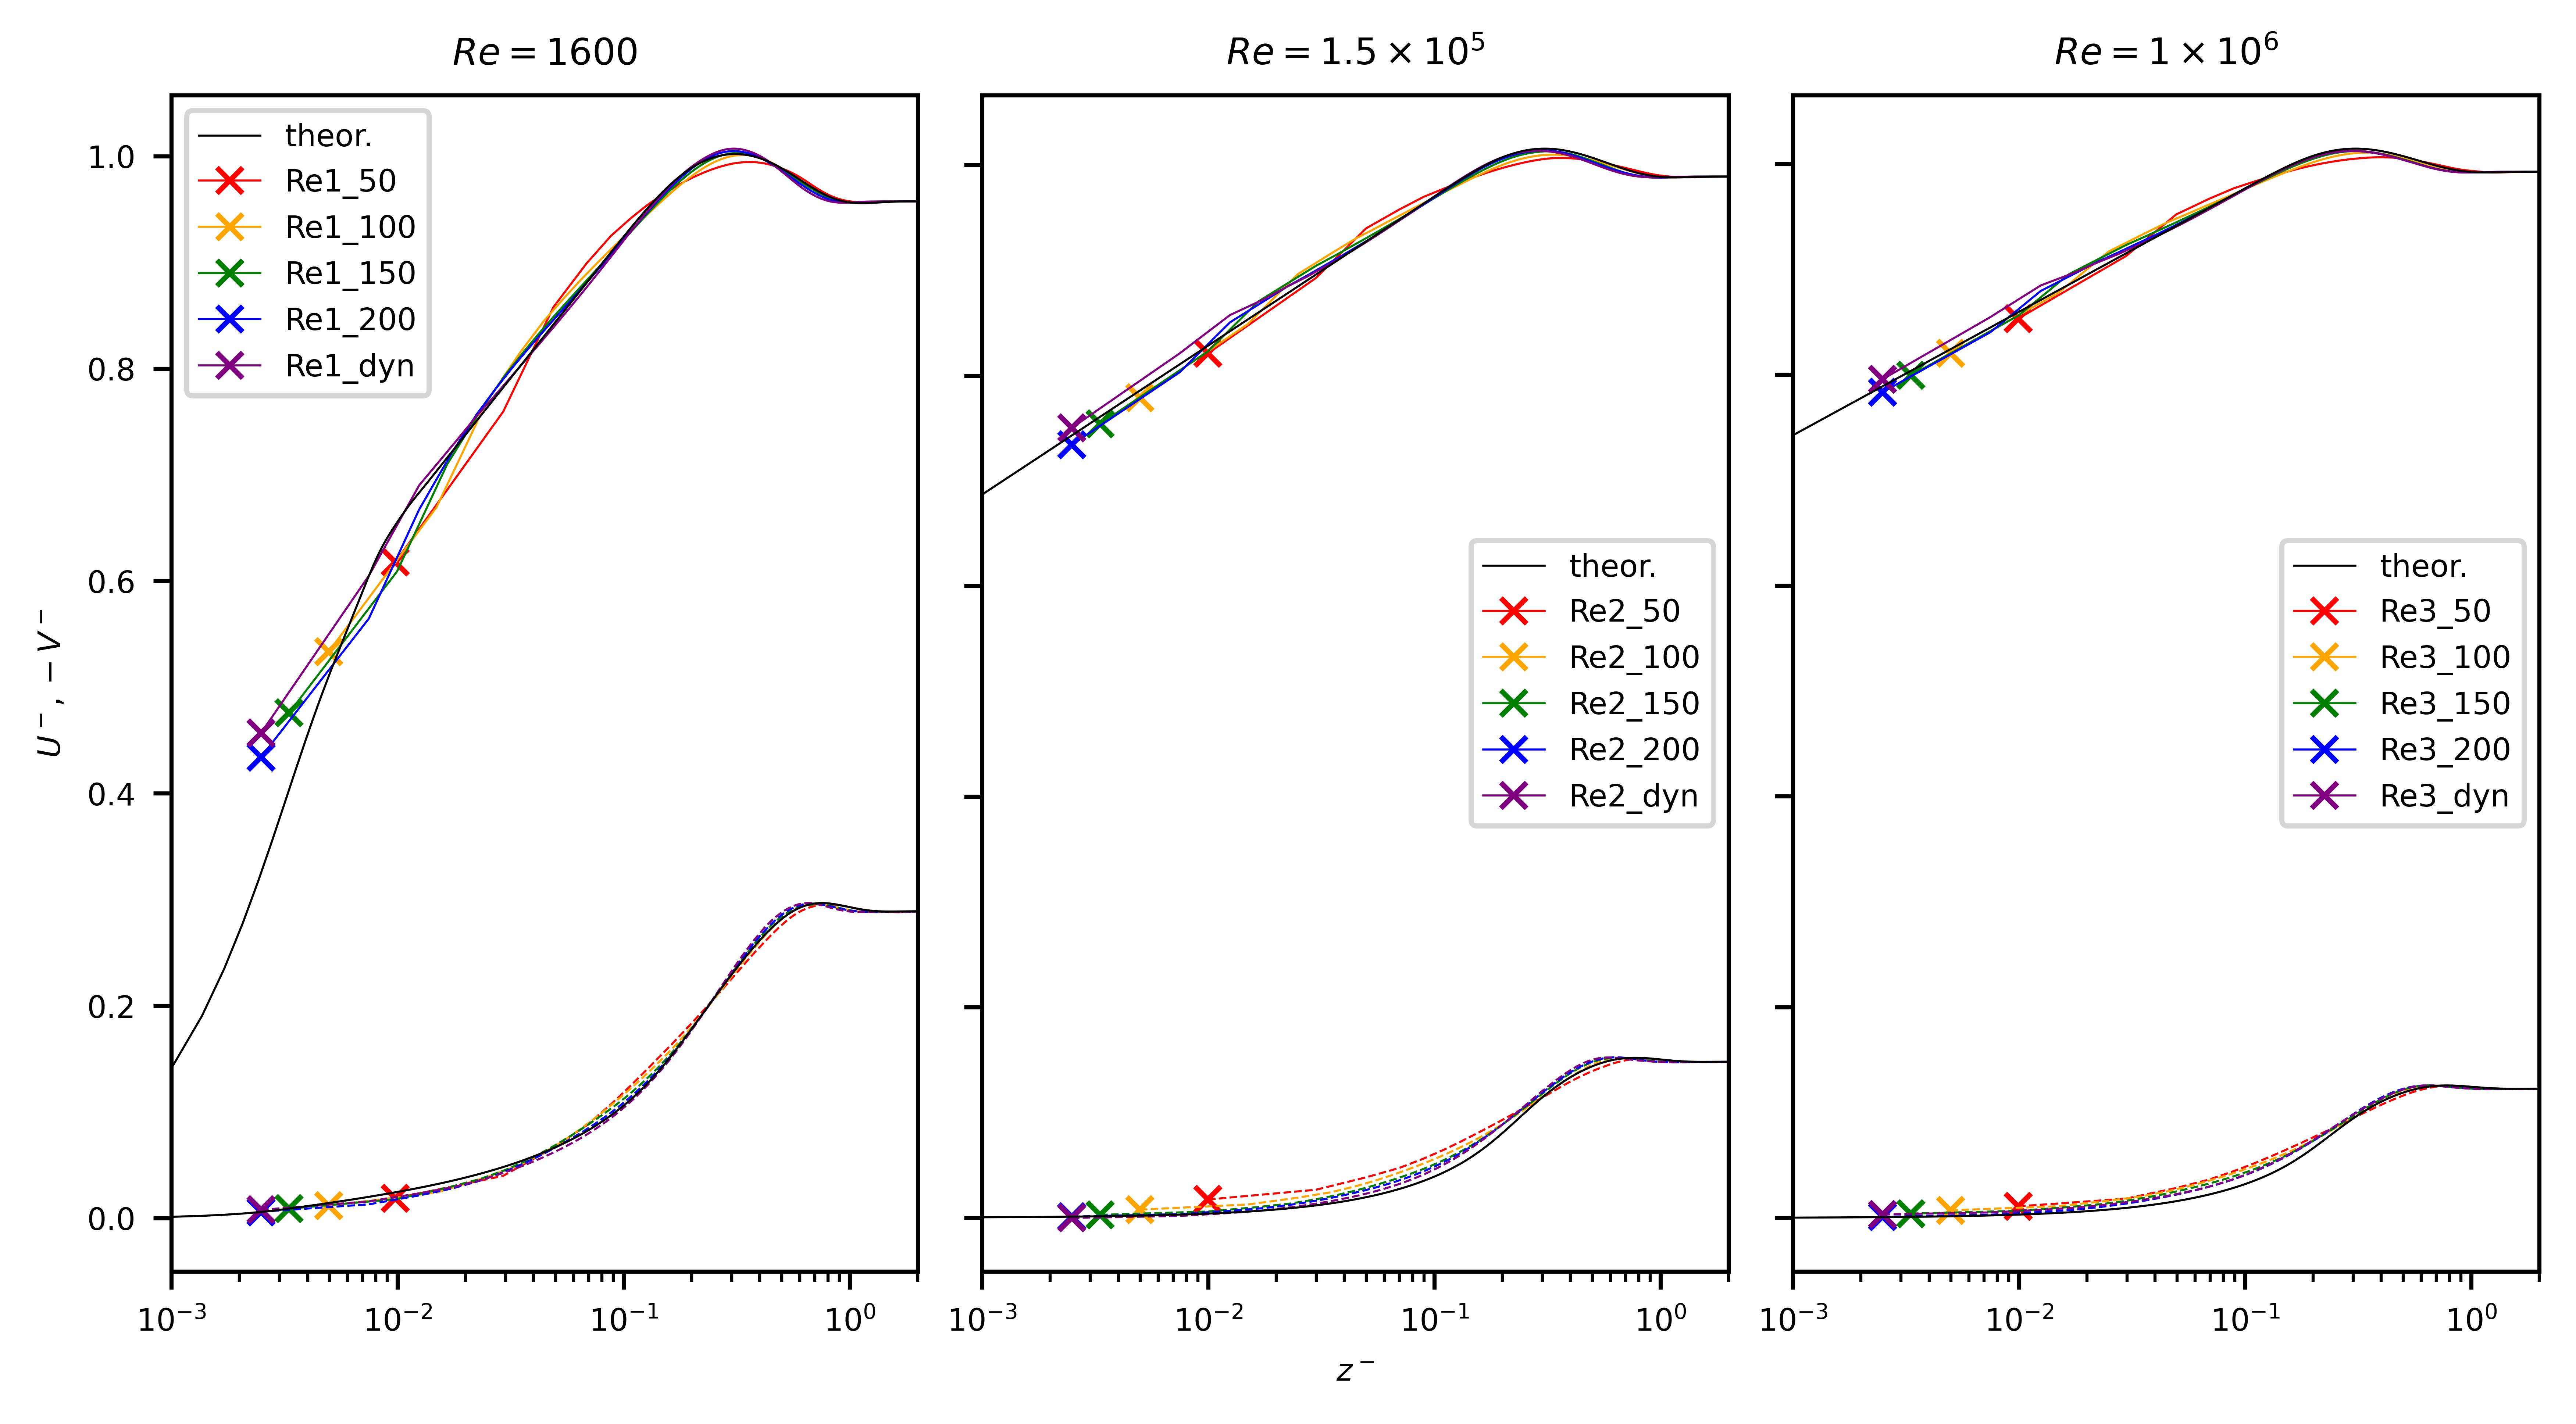
\includegraphics[width=\textwidth]{figures_2024/d3y_3Re_profiles_outer.png}
	}
  \caption{Shear-aligned velocity profiles in outer scaling. Solid lines: u-component, dashed lines: v-component. The lowest grid point is marked by \DIFdelbeginFL \DIFdelFL{$x$}\DIFdelendFL \DIFaddbeginFL \DIFaddFL{a cross ($\times$) colored according to the corresponding resolution.}\DIFaddendFL }
  \label{velocity_outer}
\end{figure}

% profiles
\DIFdelbegin \DIFdel{Figure \ref{velocity_outer} shows the velocity profiles from the LES and the theoretical profiles for each of the }\DIFdelend \DIFaddbegin \DIFadd{Velocity profiles from LES and our theoretical framework agree well for the different }\DIFaddend $\RE$ \DIFdelbegin \DIFdel{. In general, the velocity profiles of the LES agree well with the theoretical profiles: The course of the theoretical Ekman layer is matched and the simulations exhibit }\DIFdelend \DIFaddbegin \DIFadd{in Fig.\,\ref{velocity_outer}: Most prominently, the rotation across the Ekman layer agrees and }\DIFaddend a logarithmic layer for the U-component \DIFaddbegin \DIFadd{is present}\DIFaddend . The lowest points of the LES of the higher $\RE$ fall into the logarithmic layer. For Re1, the lowest grid point falls into the buffer layer, which is visible as the curved course of the U-component below the logarithmic layer in the theoretical profile. The best resolved simulation with Deardorff-closure even seems to follow the course of the upper part of the buffer layer, but with a resolution of $\Delta^+=15$ this is a coincidence caused by a well-known S-shape of velocity profiles close to rigid \DIFdelbegin \DIFdel{walls \mbox{%DIFAUXCMD
\cite{brasseur2010designing}}\hspace{0pt}%DIFAUXCMD
}\DIFdelend \DIFaddbegin \DIFadd{wall \mbox{%DIFAUXCMD
\citep{brasseur2010designing}}\hspace{0pt}%DIFAUXCMD
}\DIFaddend . This log-layer mismatch arises from a competition between the scales $u_\star$ and $z$ and other velocity and length scales introduced by the discretization of the dynamical system \citep{mason1992stochastic,brasseur2010designing}. In other words, at the lower boundary, the relevant eddies are too small to be resolved by the grid and their contribution to the flow has to be modeled. Also the vertical component is \DIFdelbegin \DIFdel{massively }\DIFdelend restricted by the \DIFdelbegin \DIFdel{non-permeability of the wall}\DIFdelend \DIFaddbegin \DIFadd{wall's impermeability}\DIFaddend , known as blocking \DIFdelbegin \DIFdel{effect. On the contrary, the SGS-closure assumes isotropic turbulence, which is not the case on the grid scale }\DIFdelend \DIFaddbegin \DIFadd{effect-- both effects illustrate a violation of isotropy }\DIFaddend near the wall \DIFaddbegin \DIFadd{and thus counter the SGS-closure assumptions}\DIFaddend .

\begin{figure}[ht]
  \centerline{
	  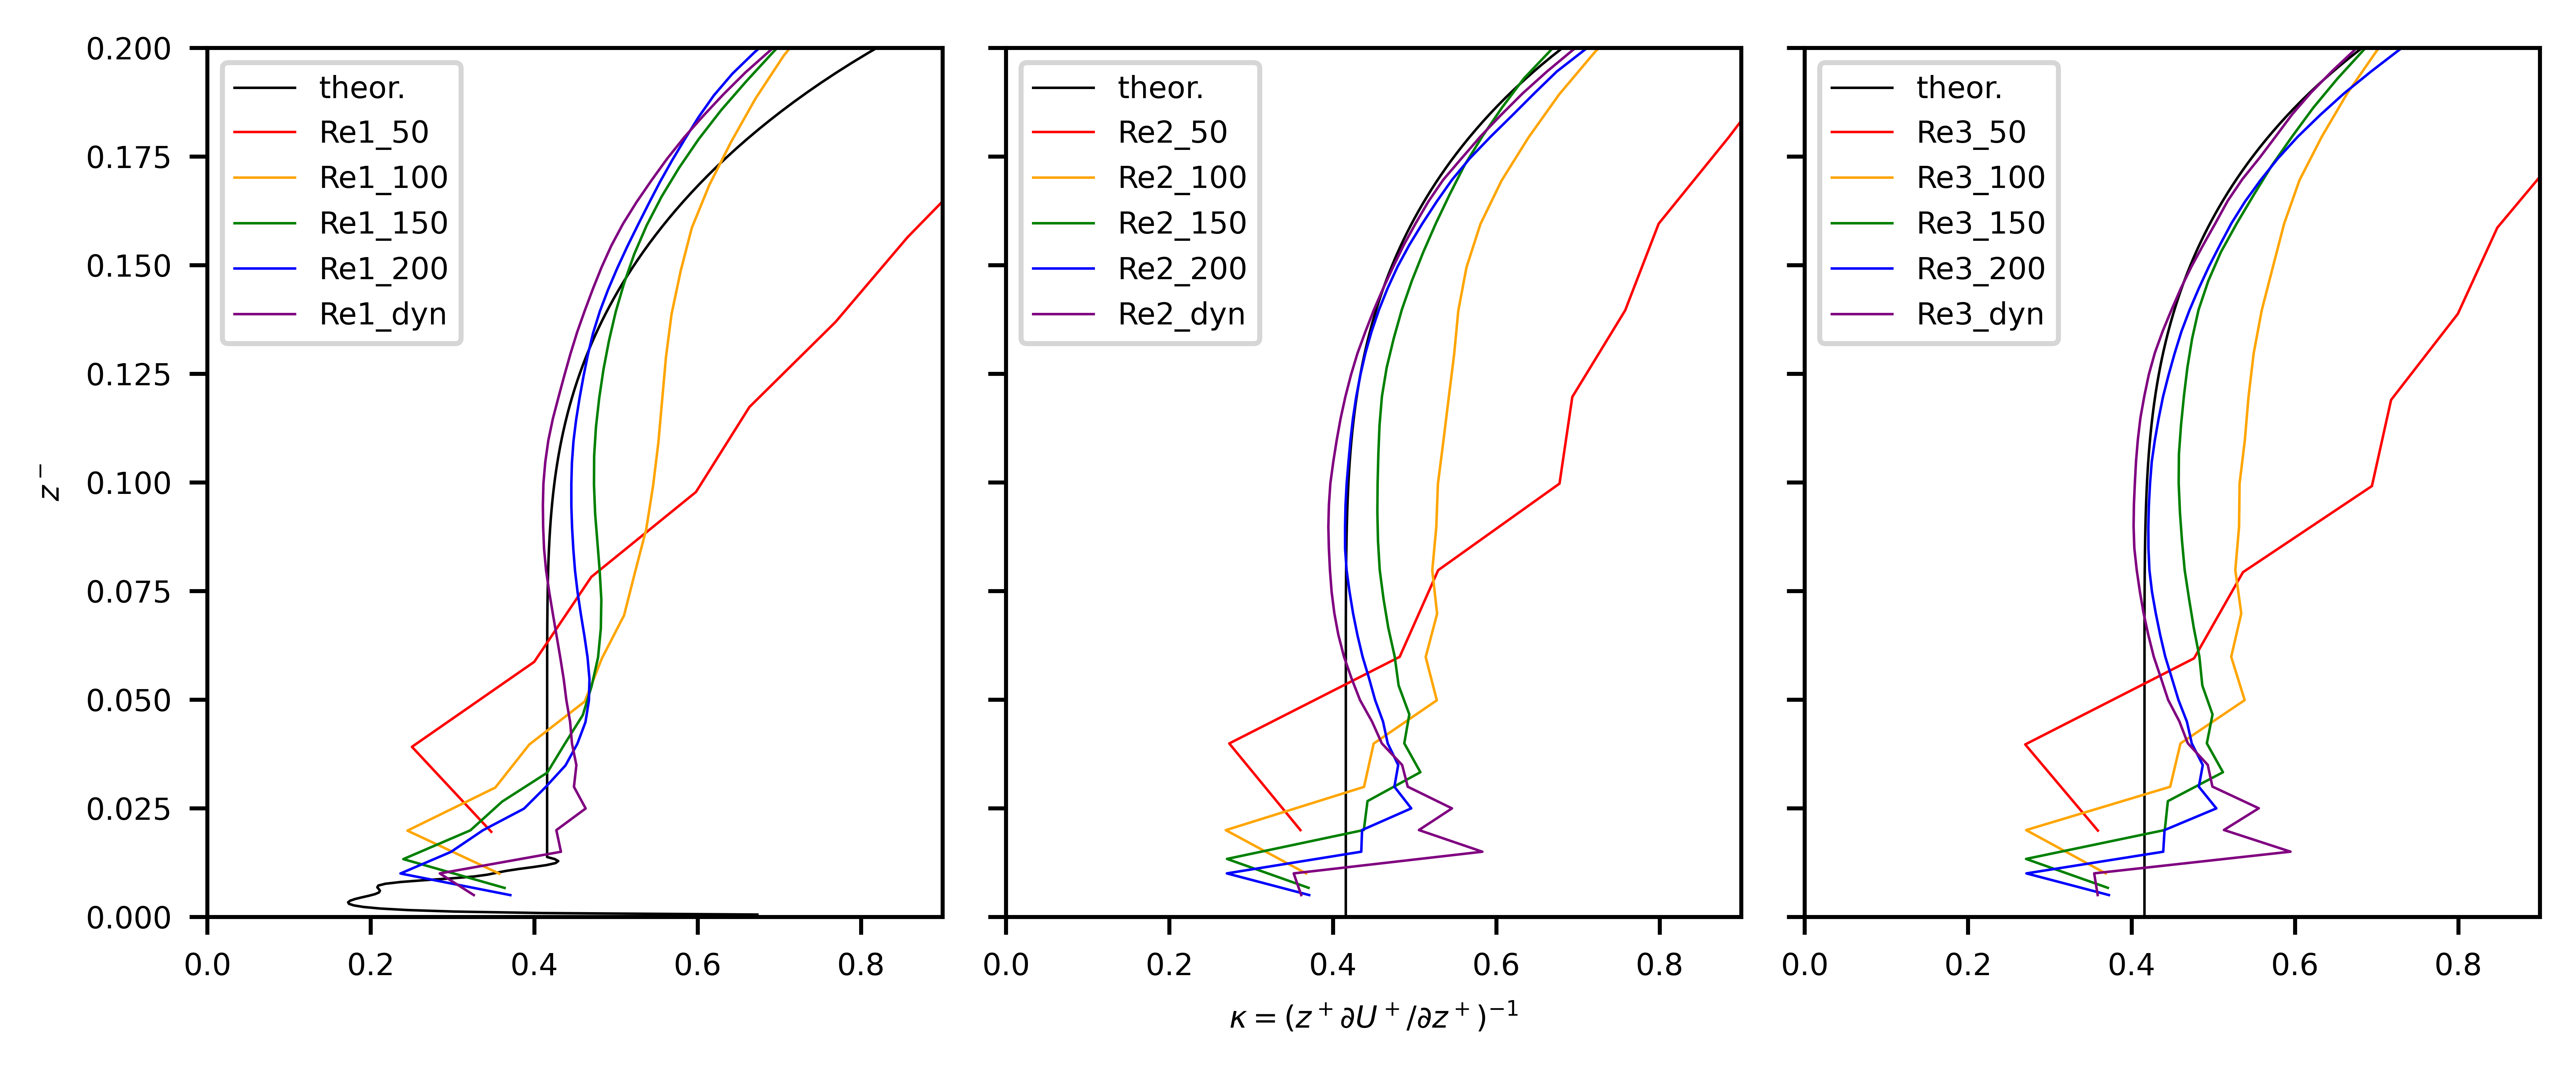
\includegraphics[width=\textwidth]{figures_2024/d3y_3Re_kappa}
  }
  \caption{K\'arm\'an measure $\kappa$ in the logarithmic region and above for different Reynolds numbers and resolutions}
  \DIFdelbeginFL %DIFDELCMD < \label{3Re_kappa}
%DIFDELCMD < %%%
\DIFdelendFL \DIFaddbeginFL \label{fig:3Re_kappa}
\DIFaddendFL \end{figure}

% kappa
\DIFdelbegin \DIFdel{In the logarithmic region, the profile of the u-component should follow the logarithmic law of eq. \ref{log-law} with the K\'arm\'an measure $\kappa = (z^+\partial U^+/\partial z^+)^{-1}=const.$. In the low-Reynolds-number case, the viscous sublayer represents about $0.5\%$ of the boundary layer, while this layer is not visible for the high-Reynolds-number cases, where the share drops to $~10^{-5}-10^{-7}$.Above the viscous sublayer, the theoretical profile shows a near-constant value for $\kappa$ up to $z^-\approx0.1$ for the case Re1 and up to $z^-\approx0.12$ for the cases Re2 and Re3.In order to estimate $\kappa_{LES}$ from the simulations, we perform a }\DIFdelend \DIFaddbegin \DIFadd{The goodness-of-fit in the loga\-rith\-mic layer (Eq.\,\ref{eqn:log-law}) is assessed through the von-K\'ar\-m\'an mea\-sure (Fig.\,\ref{fig:3Re_kappa})
}\begin{align}
  \DIFadd{\kappa(z)=(z^+\partial U^+/\partial z^+)^{-1}\simeq const.,
}\end{align}
\DIFadd{which is estimated here by }\DIFaddend linear regression of the mean velocity in x-direction \DIFdelbegin \DIFdel{and }\DIFdelend \DIFaddbegin \DIFadd{against }\DIFaddend the logarithm of height between the seventh grid point and the \DIFdelbegin \DIFdel{grid point corresponding to the height }\DIFdelend $z^-=0.1$ for \DIFdelbegin \DIFdel{$Re1\_X$ }\DIFdelend \DIFaddbegin \DIFadd{Re1 }\DIFaddend and $z^-=0.12$ for \DIFdelbegin \DIFdel{$Re2\_X$ and $Re3\_X$. We consider only points above the 7th grid point following arguments of \mbox{%DIFAUXCMD
\cite{maronga2020improved}}\hspace{0pt}%DIFAUXCMD
, that }\DIFdelend \DIFaddbegin \DIFadd{Re2 and Re3. The seventh grid point is chosen as lower boundary for the logarithmic layer as, }\DIFaddend in PALM, the mean velocity \DIFdelbegin \DIFdel{profiles follow MOST above the seventh grid point}\DIFdelend \DIFaddbegin \DIFadd{profile follows MOST aloft \mbox{%DIFAUXCMD
\citep{maronga2020improved}}\hspace{0pt}%DIFAUXCMD
}\DIFaddend . The number of values for each regression is 6, 12, and 18 for \DIFdelbegin \DIFdel{$ReX\_100$, $ReX\_150$ and $ReX\_200$}\DIFdelend \DIFaddbegin \DIFadd{ReX\_100, ReX\_150 and ReX\_200}\DIFaddend , respectively.  \DIFaddbegin \DIFadd{In case Re1, the viscous sublayer occupies about $0.5\%$ of the boundary layer, but this share drops to $~10^{-5}-10^{-7}$ for cases Re2 and Re3 respectively. Above the viscous sublayer, the theoretical profile shows a near-constant value for $\kappa$ up to $z^-\approx0.1$ for the case Re1 and up to $z^-\approx0.12$ for the cases Re2 and Re3. }\DIFaddend We do not compute $\kappa$ for \DIFdelbegin \DIFdel{$ReX\_50$ }\DIFdelend \DIFaddbegin \DIFadd{ReX\_50 }\DIFaddend since there are only six grid points below $z^-\approx 0.12$\DIFaddbegin \DIFadd{, and o constant K\'arm\'an measure $\kappa(z)$ can be observed}\DIFaddend . The resulting \DIFdelbegin \DIFdel{$\kappa_{LES}$ for the other simulations }\DIFdelend \DIFaddbegin \DIFadd{best estimates for $\kappa_{LES}$ }\DIFaddend are shown in \DIFdelbegin \DIFdel{Tbl.\ref{simulation_results}. The }\DIFdelend \DIFaddbegin \DIFadd{Tab.\,\ref{simulation_results}, where the }\DIFaddend coefficient of determination \DIFaddbegin \DIFadd{('r-squared') }\DIFaddend is above 0.99 for all \DIFdelbegin \DIFdel{fits. 
}\DIFdelend \DIFaddbegin \DIFadd{cases. 
}

\DIFadd{For finer resolution, }\DIFaddend $\kappa_{LES}$ \DIFdelbegin \DIFdel{is decreasing with finer resolutionfor all $\RE$. While the values for $ReX\_100$ are rather high with }\DIFdelend \DIFaddbegin \DIFadd{decreases with increasing Re for the range of scale separation investigated here. ReX\_100 yields }\DIFaddend a value around $0.53$ \DIFdelbegin \DIFdel{, finer resolution leads to values closer to measurements }\DIFdelend \DIFaddbegin \DIFadd{(which is outside the range agreed on by atmospheric observation and laboratory measurements), the finer resolution yields values }\DIFaddend around $0.46$ for \DIFdelbegin \DIFdel{$Re1\_200$ }\DIFdelend \DIFaddbegin \DIFadd{Re1\_200 }\DIFaddend and around $0.44$ for \DIFdelbegin \DIFdel{$Re2\_200$ and $Re3\_200$}\DIFdelend \DIFaddbegin \DIFadd{Re2\_200 and Re3\_200, which is in excellenet agreement with DNS data and laboratory measurements}\DIFaddend . The dynamic subgrid closure yields lower values for $\kappa_{LES}$: in \DIFdelbegin \DIFdel{$Re1\_dyn$ }\DIFdelend \DIFaddbegin \DIFadd{Re1\_dyn }\DIFaddend we even see $\kappa_{LES}=0.39$, while \DIFdelbegin \DIFdel{$Re2\_dyn$ and $Re3\_dyn$ }\DIFdelend \DIFaddbegin \DIFadd{Re2\_dyn and Re3\_dyn }\DIFaddend yield $0.42$ and $0.43$, respectively. \DIFdelbegin \DIFdel{Figure \ref{3Re_kappa} shows the K\'arm\'an measure in the logarithmic layer. For the simulations $ReX\_50$, no constant $\kappa$ can be observed. An increase in resolution leads to a profile of the K\'arm\'an measure closer to the theoretical curve for all cases. }\DIFdelend Close to the bottom, the K\'arm\'an measure is heavily influenced by the proximity of the wall and rather a function of the vertical index than of the physical distance from the wall. In accordance with \DIFdelbegin \DIFdel{the observations of }\DIFdelend \cite{maronga2014monin} and \cite{maronga2017formulation}, the kinks in the K\'arm\'an measure diminish around the seventh grid point for all simulations. Above, the curve smoothens and approaches the expected value of $\kappa$\DIFdelbegin \DIFdel{(at least for the finer resolutions)}\DIFdelend .  

\begin{figure}[ht]
  \DIFdelbeginFL %DIFDELCMD < \centerline{
%DIFDELCMD < 	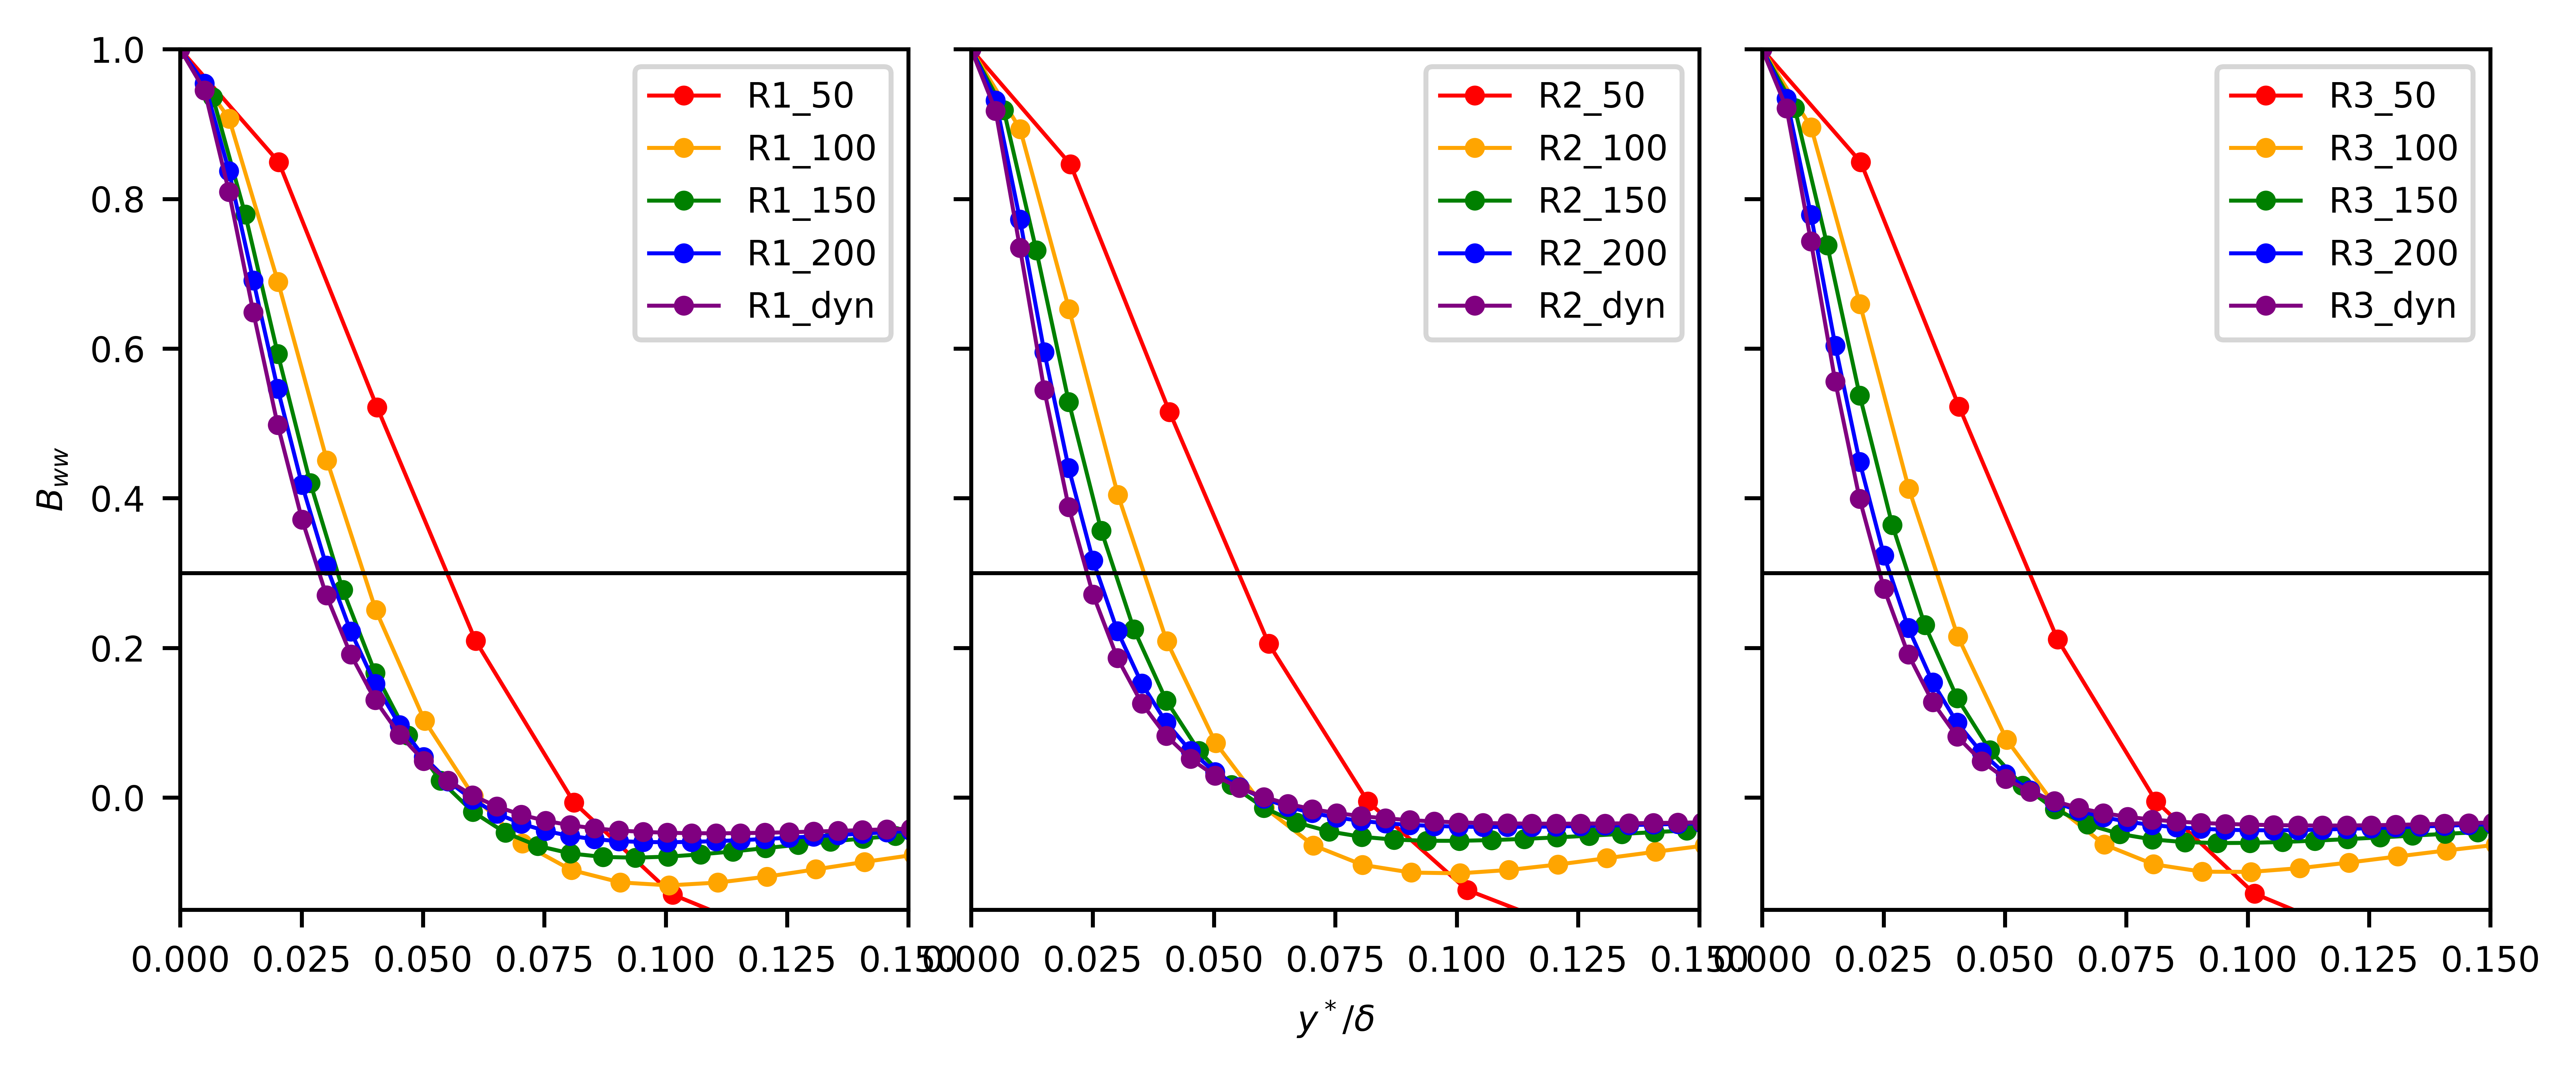
\includegraphics[width=\textwidth]{figures_2024/d3y_2pc_ww_3Re_0.079.png}
%DIFDELCMD < }
%DIFDELCMD <   %%%
\DIFdelendFL \DIFaddbeginFL \centerline{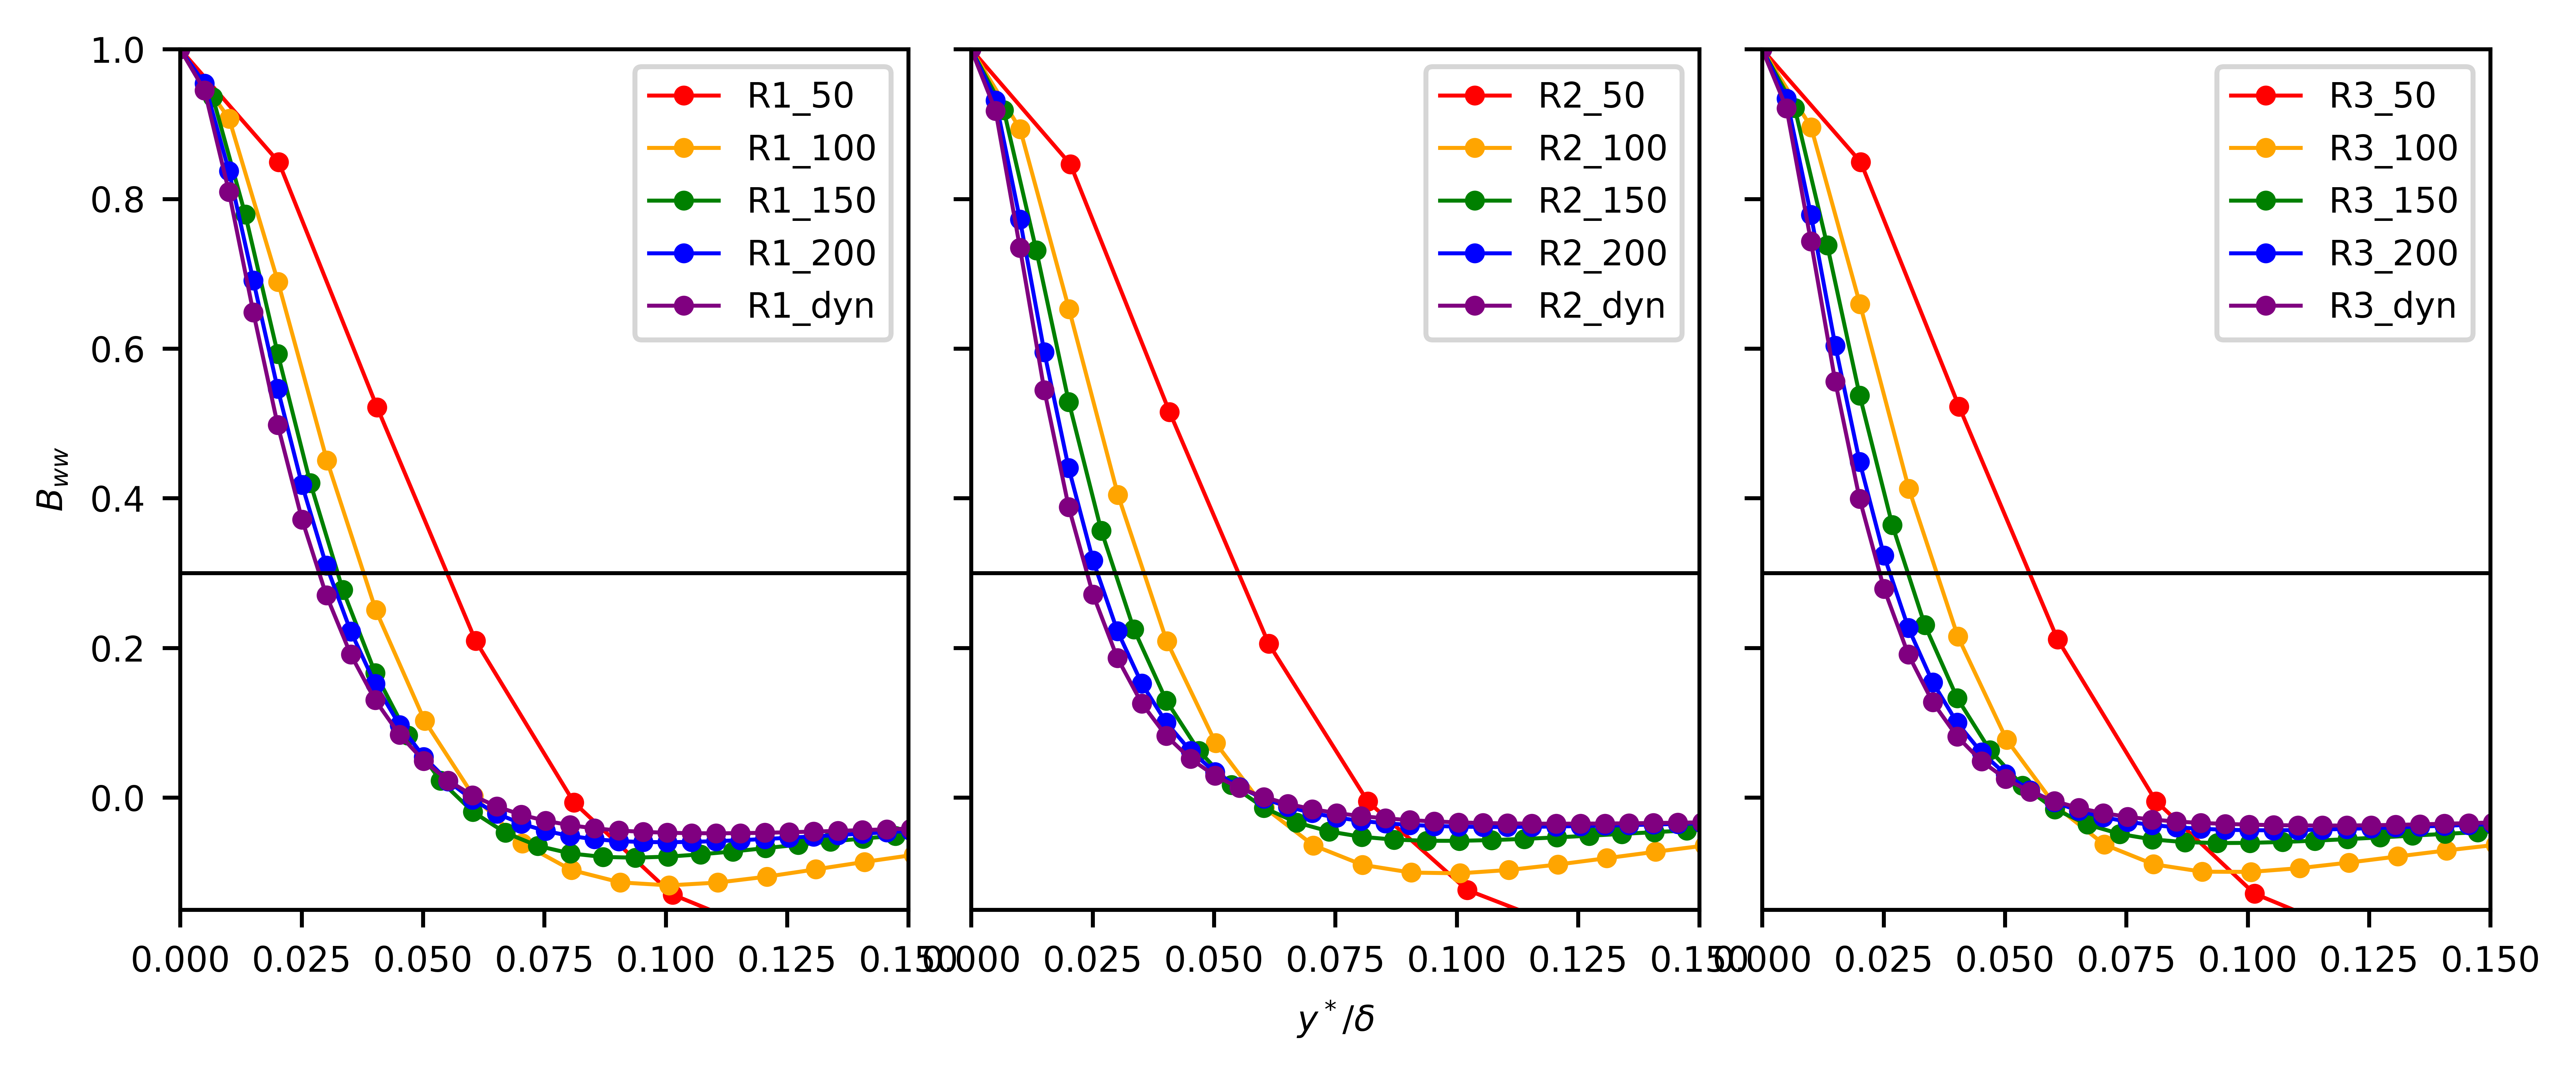
\includegraphics[width=\textwidth]{figures_2024/d3y_2pc_ww_3Re_0.079.png}}
  \DIFaddendFL \caption{Two-point correlation of w-component in y-direction at $z^-\approx 0.08$. The horizontal line \DIFdelbeginFL \DIFdelFL{is }\DIFdelendFL at $B_{ww}=0.3$ \DIFaddbeginFL \DIFaddFL{is indicative of the average size of turbulent structures in the flow.}\DIFaddendFL }
  \DIFdelbeginFL %DIFDELCMD < \label{2pc_008}
%DIFDELCMD < %%%
\DIFdelendFL \DIFaddbeginFL \label{fig:2pc_008}
\DIFaddendFL \end{figure}

\DIFdelbegin \DIFdel{As expected }\DIFdelend \DIFaddbegin \DIFadd{The resolution near the surface is critical }\DIFaddend for an LES with isotropic grid spacing\DIFdelbegin \DIFdel{, the resolution near the surface is a critical part of the simulation. We can support our above observations by taking a look at the }\DIFdelend \DIFaddbegin \DIFadd{. \todo{Missing transition from resolution to two-point correlation!} The }\DIFaddend two-point \DIFdelbegin \DIFdel{correlation in the critical layers of the simulations. The two point }\DIFdelend correlation is defined as 
\DIFdelbegin \begin{align*}
  \DIFdel{B_{xx}\left(x^*\right) = \langle u\left(x-x^*\right)u\left(x\right)\rangle/\sigma_u^2.
}\end{align*}%DIFAUXCMD
\DIFdelend \DIFaddbegin \begin{align}
  \DIFadd{B_{xx}\left(x^*\right) = \langle u\left(x-x^*\right)u\left(x\right)\rangle/\sigma_u^2,
}\end{align}\DIFaddend 
\DIFdelbegin \DIFdel{As suggested by \mbox{%DIFAUXCMD
\cite{wurps2020grid}}\hspace{0pt}%DIFAUXCMD
, in an isotropic grid with periodic horizontal boundary conditions the turbulent structures of the velocity's w-component in y-direction can serve as an indicator }\DIFdelend \DIFaddbegin \DIFadd{and it supports the above findings \todo{which findings?}. 
For an LES with isotropic grid and periodic horizontal boundaries, the the span-wise two-point correlation of the vertical velocity component $B_{ww}(y^*)$ indicates }\DIFaddend how well the flow is resolved \DIFdelbegin \DIFdel{. Figure \ref{2pc_008} shows the two-point correlation $B_{ww}(y^*)$ at a height of $z^-\approx 0.08$, which is right inside of the logarithmic layer}\DIFdelend \DIFaddbegin \DIFadd{\mbox{%DIFAUXCMD
\citep{wurps2020grid}}\hspace{0pt}%DIFAUXCMD
}\DIFaddend . We define \DIFaddbegin \DIFadd{$\sigma$, }\DIFaddend the average size of a structure in the flow\DIFdelbegin \DIFdel{$\sigma$ as the distance where }\DIFdelend \DIFaddbegin \DIFadd{, as the separation at which }\DIFaddend the two-point correlation \DIFaddbegin \DIFadd{at a height $z^-\approx 0.08$, right inside the logarithmic layer, }\DIFaddend drops to 0.3\DIFdelbegin \DIFdel{(horizontal line in figure}\DIFdelend \DIFaddbegin \DIFadd{, i.e. $B_{ww}(\sigma^\star) = 0.3$ (Fig.\,\ref{fig:2pc_008}}\DIFaddend ). The number of cells by which the \DIFdelbegin \DIFdel{average }\DIFdelend \DIFaddbegin \DIFadd{corresponding }\DIFaddend structure is resolved is \DIFdelbegin \DIFdel{equal to }\DIFdelend \DIFaddbegin \DIFadd{then }\DIFaddend $\sigma/\Delta$. All \DIFdelbegin \DIFdel{$\RE$ }\DIFdelend \DIFaddbegin \DIFadd{cases }\DIFaddend show a similar behaviour\DIFaddbegin \DIFadd{, irrespective of the Reynolds number}\DIFaddend : the average size of the structure decreases with finer resolution\DIFdelbegin \DIFdel{and seems to approach }\DIFdelend \DIFaddbegin \DIFadd{. and it approaches }\DIFaddend a limit. The structure size of \DIFaddbegin \DIFadd{cases }\DIFaddend ReX\_150 and ReX\_200 \DIFdelbegin \DIFdel{are very close together, which indicates beginning }\DIFdelend \DIFaddbegin \DIFadd{agrees well, indicating }\DIFaddend convergence. Furthermore, the number of cells by which the structures are resolved \DIFdelbegin \DIFdel{exceed 4 }\DIFdelend \DIFaddbegin \DIFadd{exceeds four }\DIFaddend from the resolution of ReX\_150 on. This corresponds to the resolution from which on a logarithmic layer with a constant $\kappa$ can be seen. It also fits to the rule of thumb given in \cite{wurps2020grid}, that in a sufficiently resolved part of an LES the average structures of the w-component in y-direction should be resolved by at least 4 cells. The dynamic closure shows structures that are slightly smaller than the structures of $ReX\_200$, which is caused by a tendency to lower eddy-viscosities and, hence, a weaker coupling of neighboring grid cells.

\begin{figure}[ht]
  \DIFdelbeginFL %DIFDELCMD < \centerline{
%DIFDELCMD < 	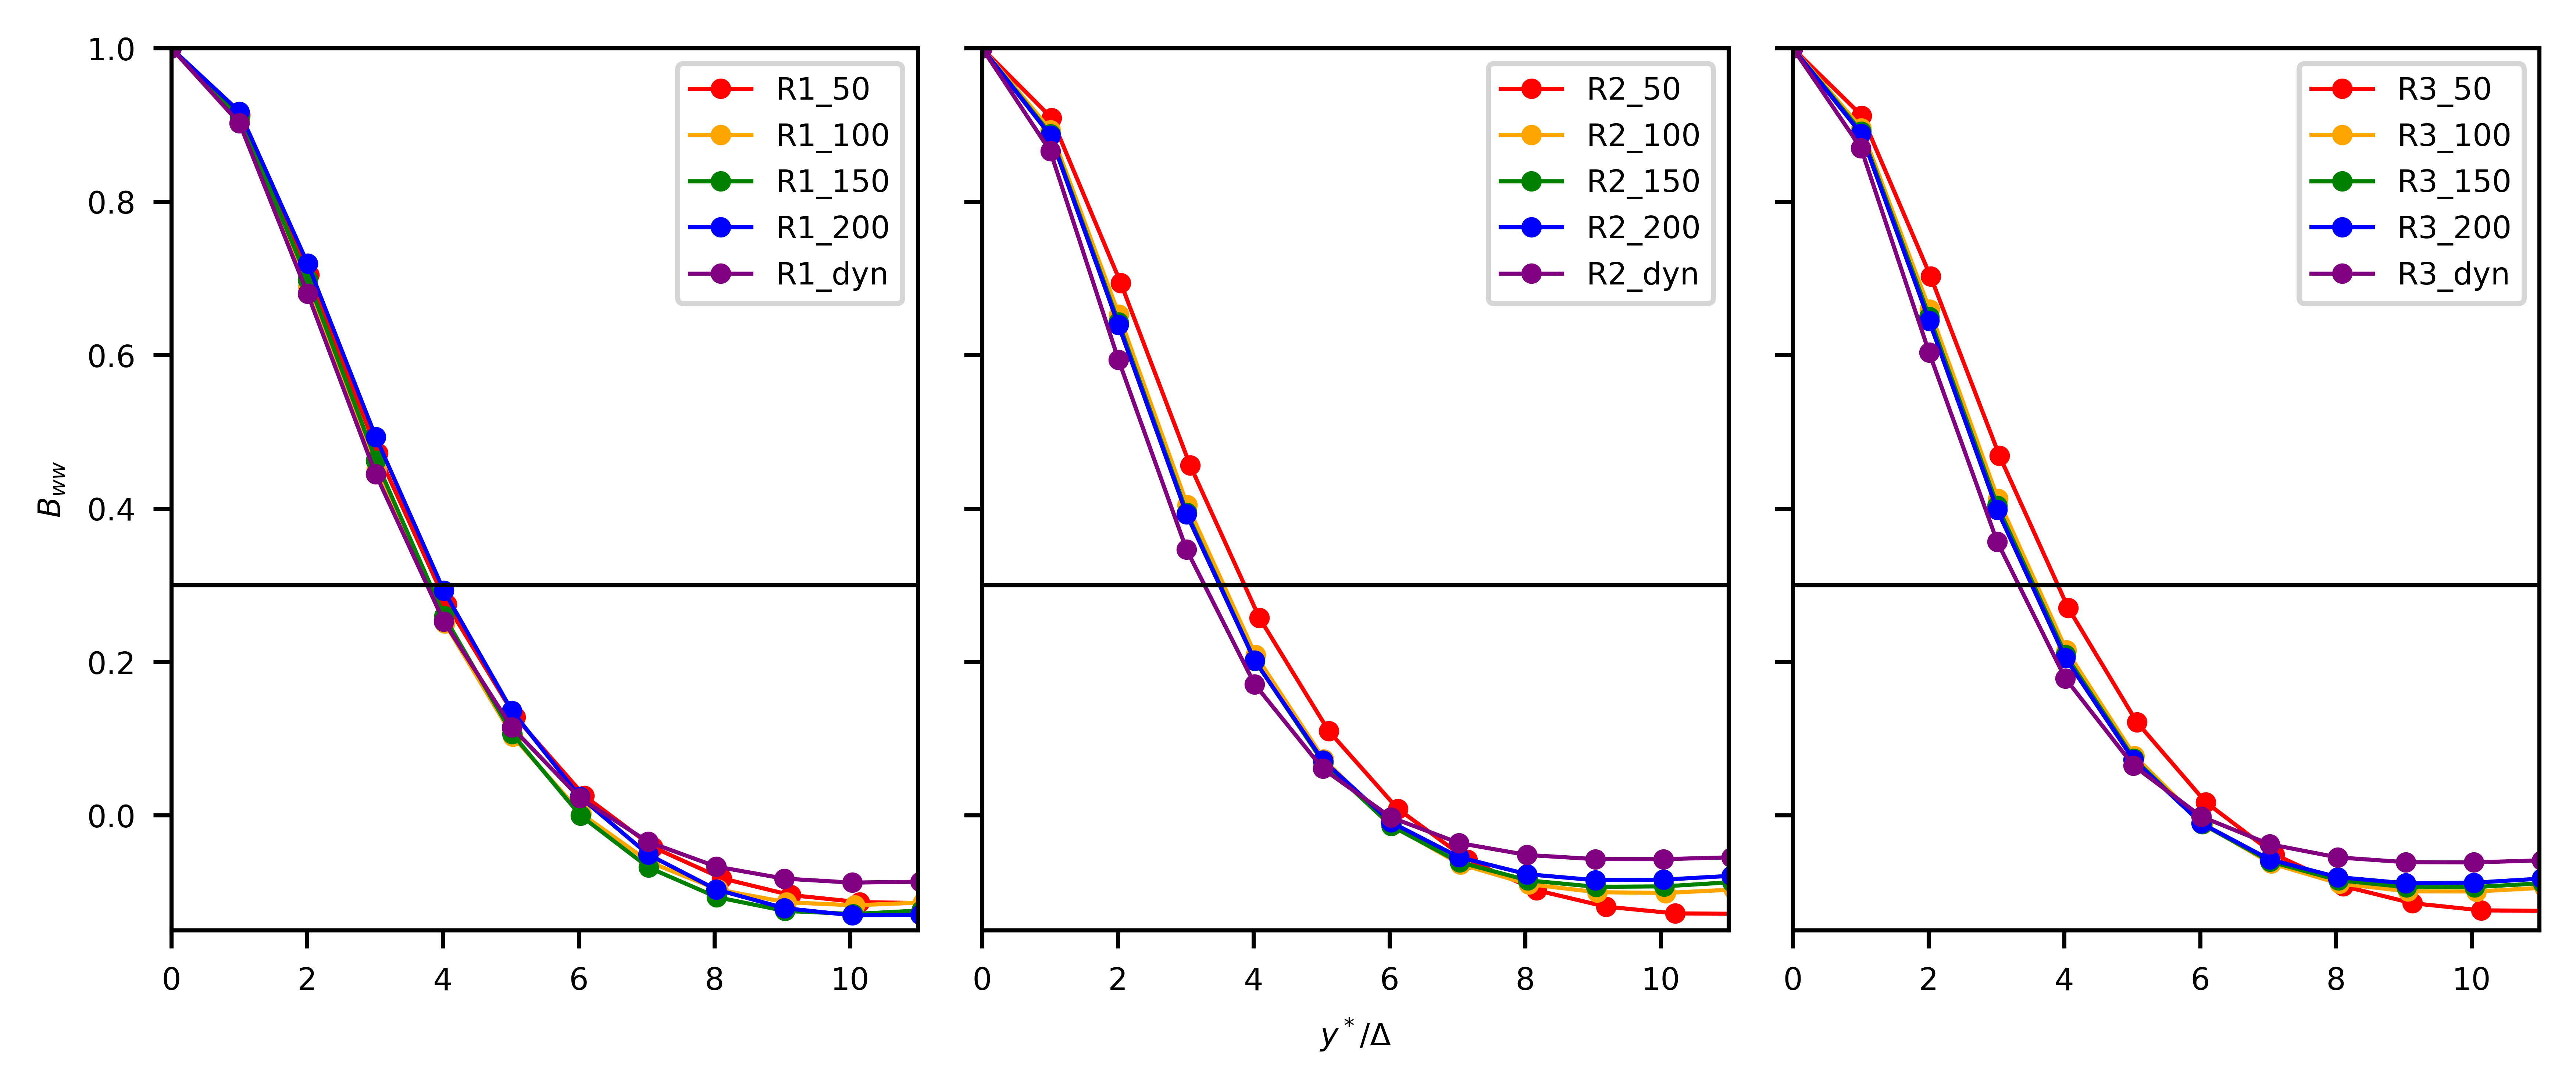
\includegraphics[width=\textwidth]{figures_2024/d3y_2pc_ww_3Re_4.png}
%DIFDELCMD < }
%DIFDELCMD <   %%%
\DIFdelendFL \DIFaddbeginFL \centerline{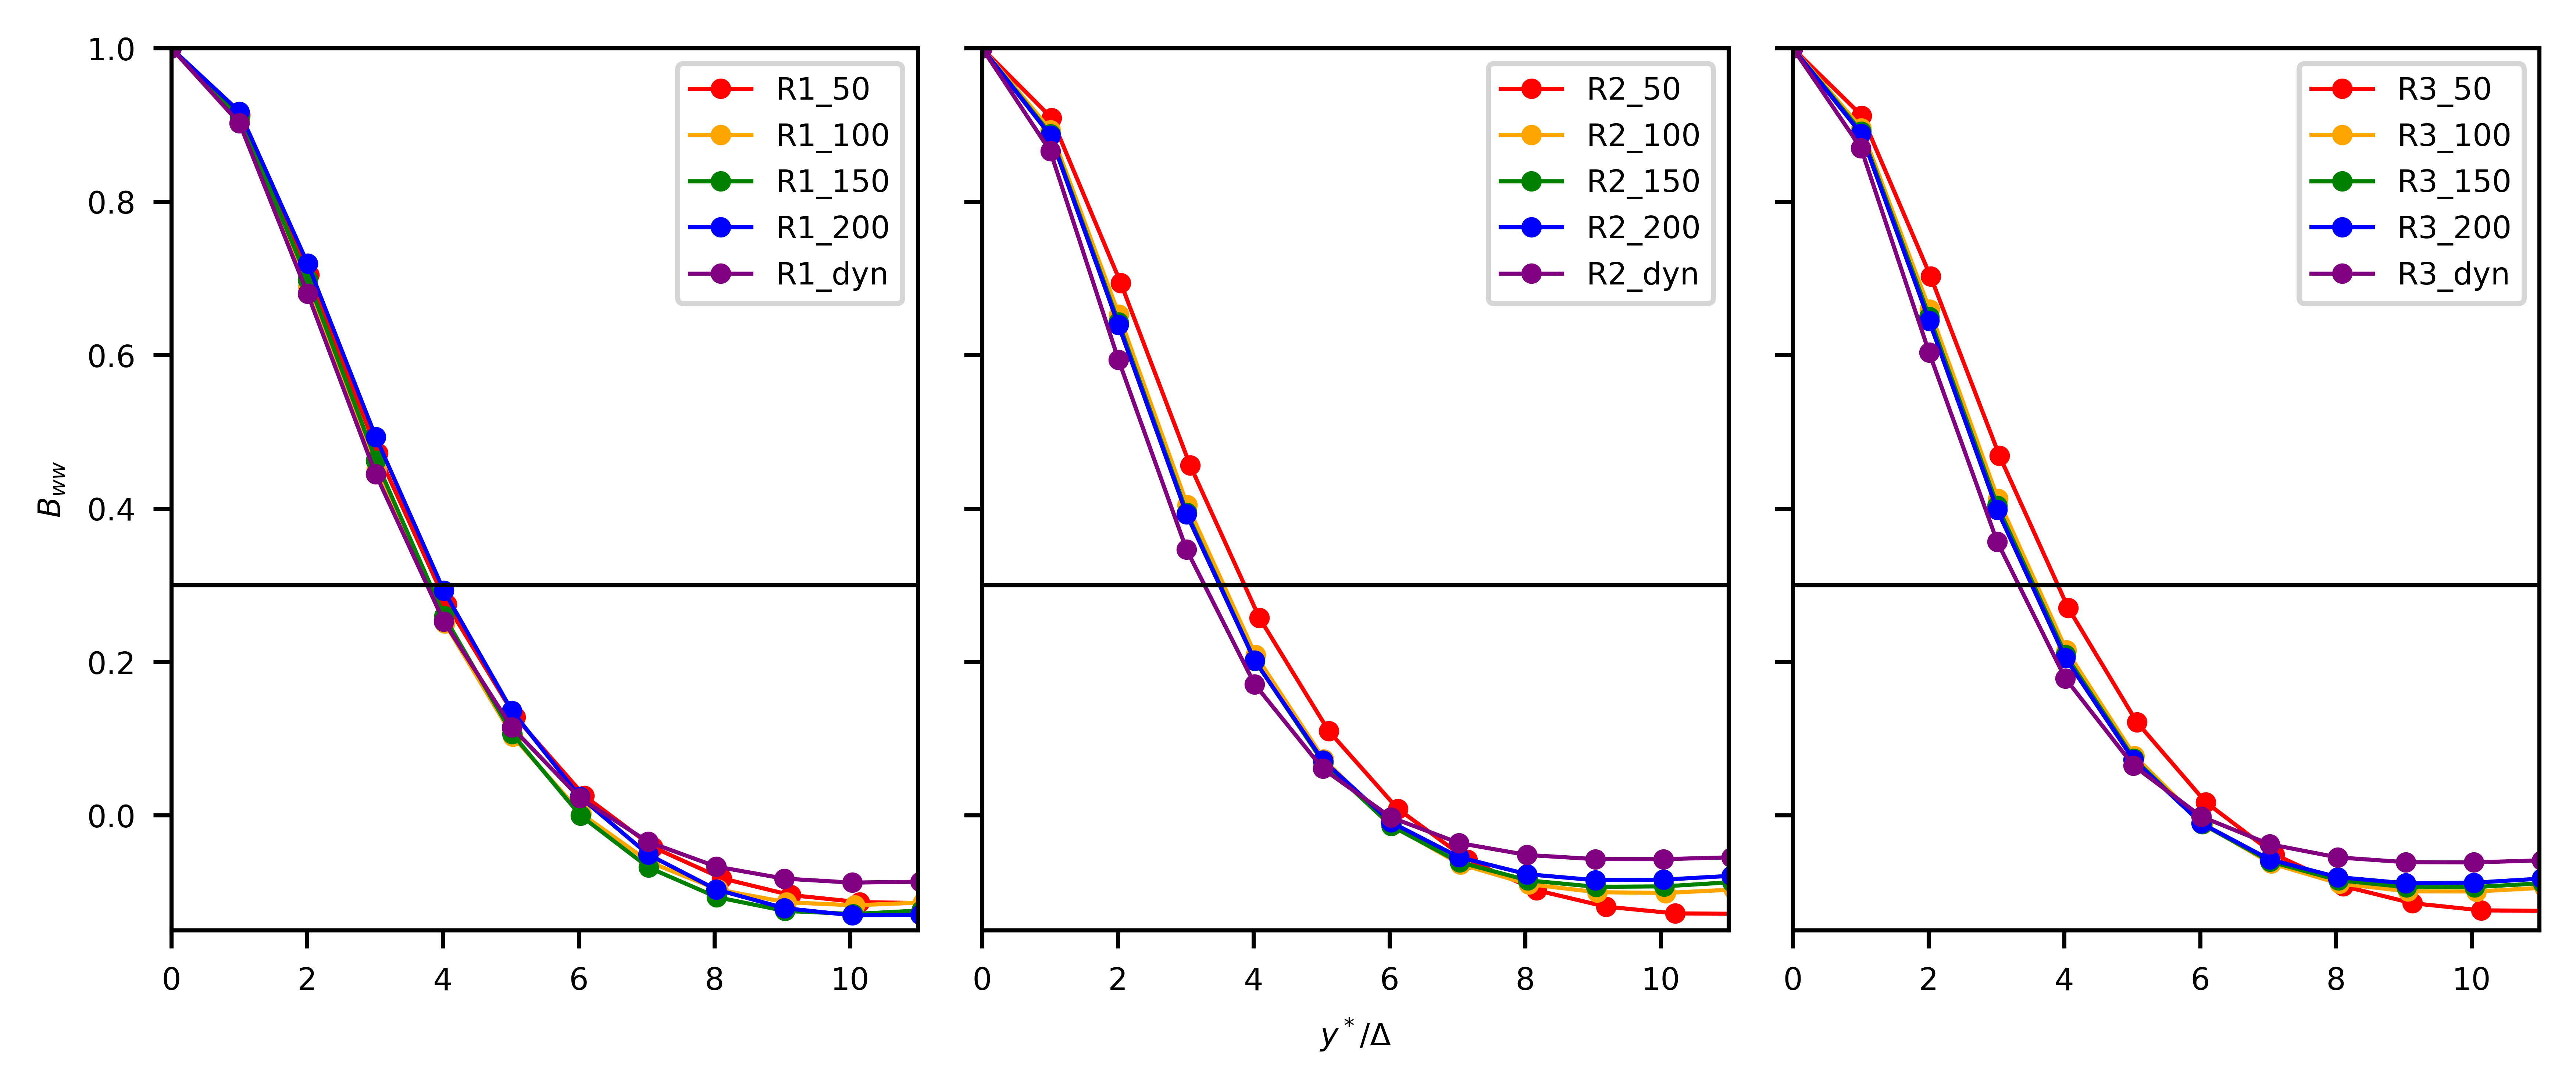
\includegraphics[width=\textwidth]{figures_2024/d3y_2pc_ww_3Re_4.png}}
  \DIFaddendFL \caption{Two-point correlation of w-component in y-direction at the 8th grid point above the surface}
  \DIFdelbeginFL %DIFDELCMD < \label{2pc_4}
%DIFDELCMD < %%%
\DIFdelendFL \DIFaddbeginFL \label{fig:2pc_4}
\DIFaddendFL \end{figure}

\DIFdelbegin \DIFdel{Figure \ref{2pc_4} shows }\DIFdelend \DIFaddbegin \DIFadd{In vicinity of the surface, the two-point statistics crucially depend on how the surface-interaction is modelled \mbox{%DIFAUXCMD
\citep{maronga2014monin}}\hspace{0pt}%DIFAUXCMD
. which may cause strong sensitivity on the resolution. Indeed, the two-point correlations }\DIFaddend $B_{ww}(y^*)$ \DIFaddbegin \DIFadd{evaluated }\DIFaddend at the 8th grid point above the bottom \DIFdelbegin \DIFdel{. Therefore, the corresponding heights differ between the simulations , that is }\DIFdelend \DIFaddbegin \DIFadd{(Fig.~\ref{fig:2pc_4}) appear rather universal. This is in spite of different heights the simulations (}\DIFaddend $z^-=0.16, 0.08, 0.053, 0.04, 0.04$ for $ReX\_50$, $ReX\_100$, $ReX\_150$, $ReX\_200$, $ReX\_dyn$, respectively\DIFaddbegin \DIFadd{)}\DIFaddend . For $Re1$, the curves almost collapse perfectly while for $Re2$ and $Re3$ we see slightly larger structures for $ReX\_50$ and slightly smaller structures for $ReX\_dyn$. This means that even 8 points above the lower boundary the smallest size of the turbulent structures rather depends on the grid cell size than on the actual height above the ground. According to the above findings and \cite{maronga2014monin}, the flow should start to be well resolved from here on (above the seventh grid point). And indeed, the number of resolving cells is very close to 4 for $Re1$ and between 3 and 4 for $Re2$ and $Re3$, which is close to the recommended 4 cells.

%
\subsection{Logarithmic layer span-wise velocity}

\begin{figure}[ht]
  \DIFdelbeginFL %DIFDELCMD < \centerline{
%DIFDELCMD < 	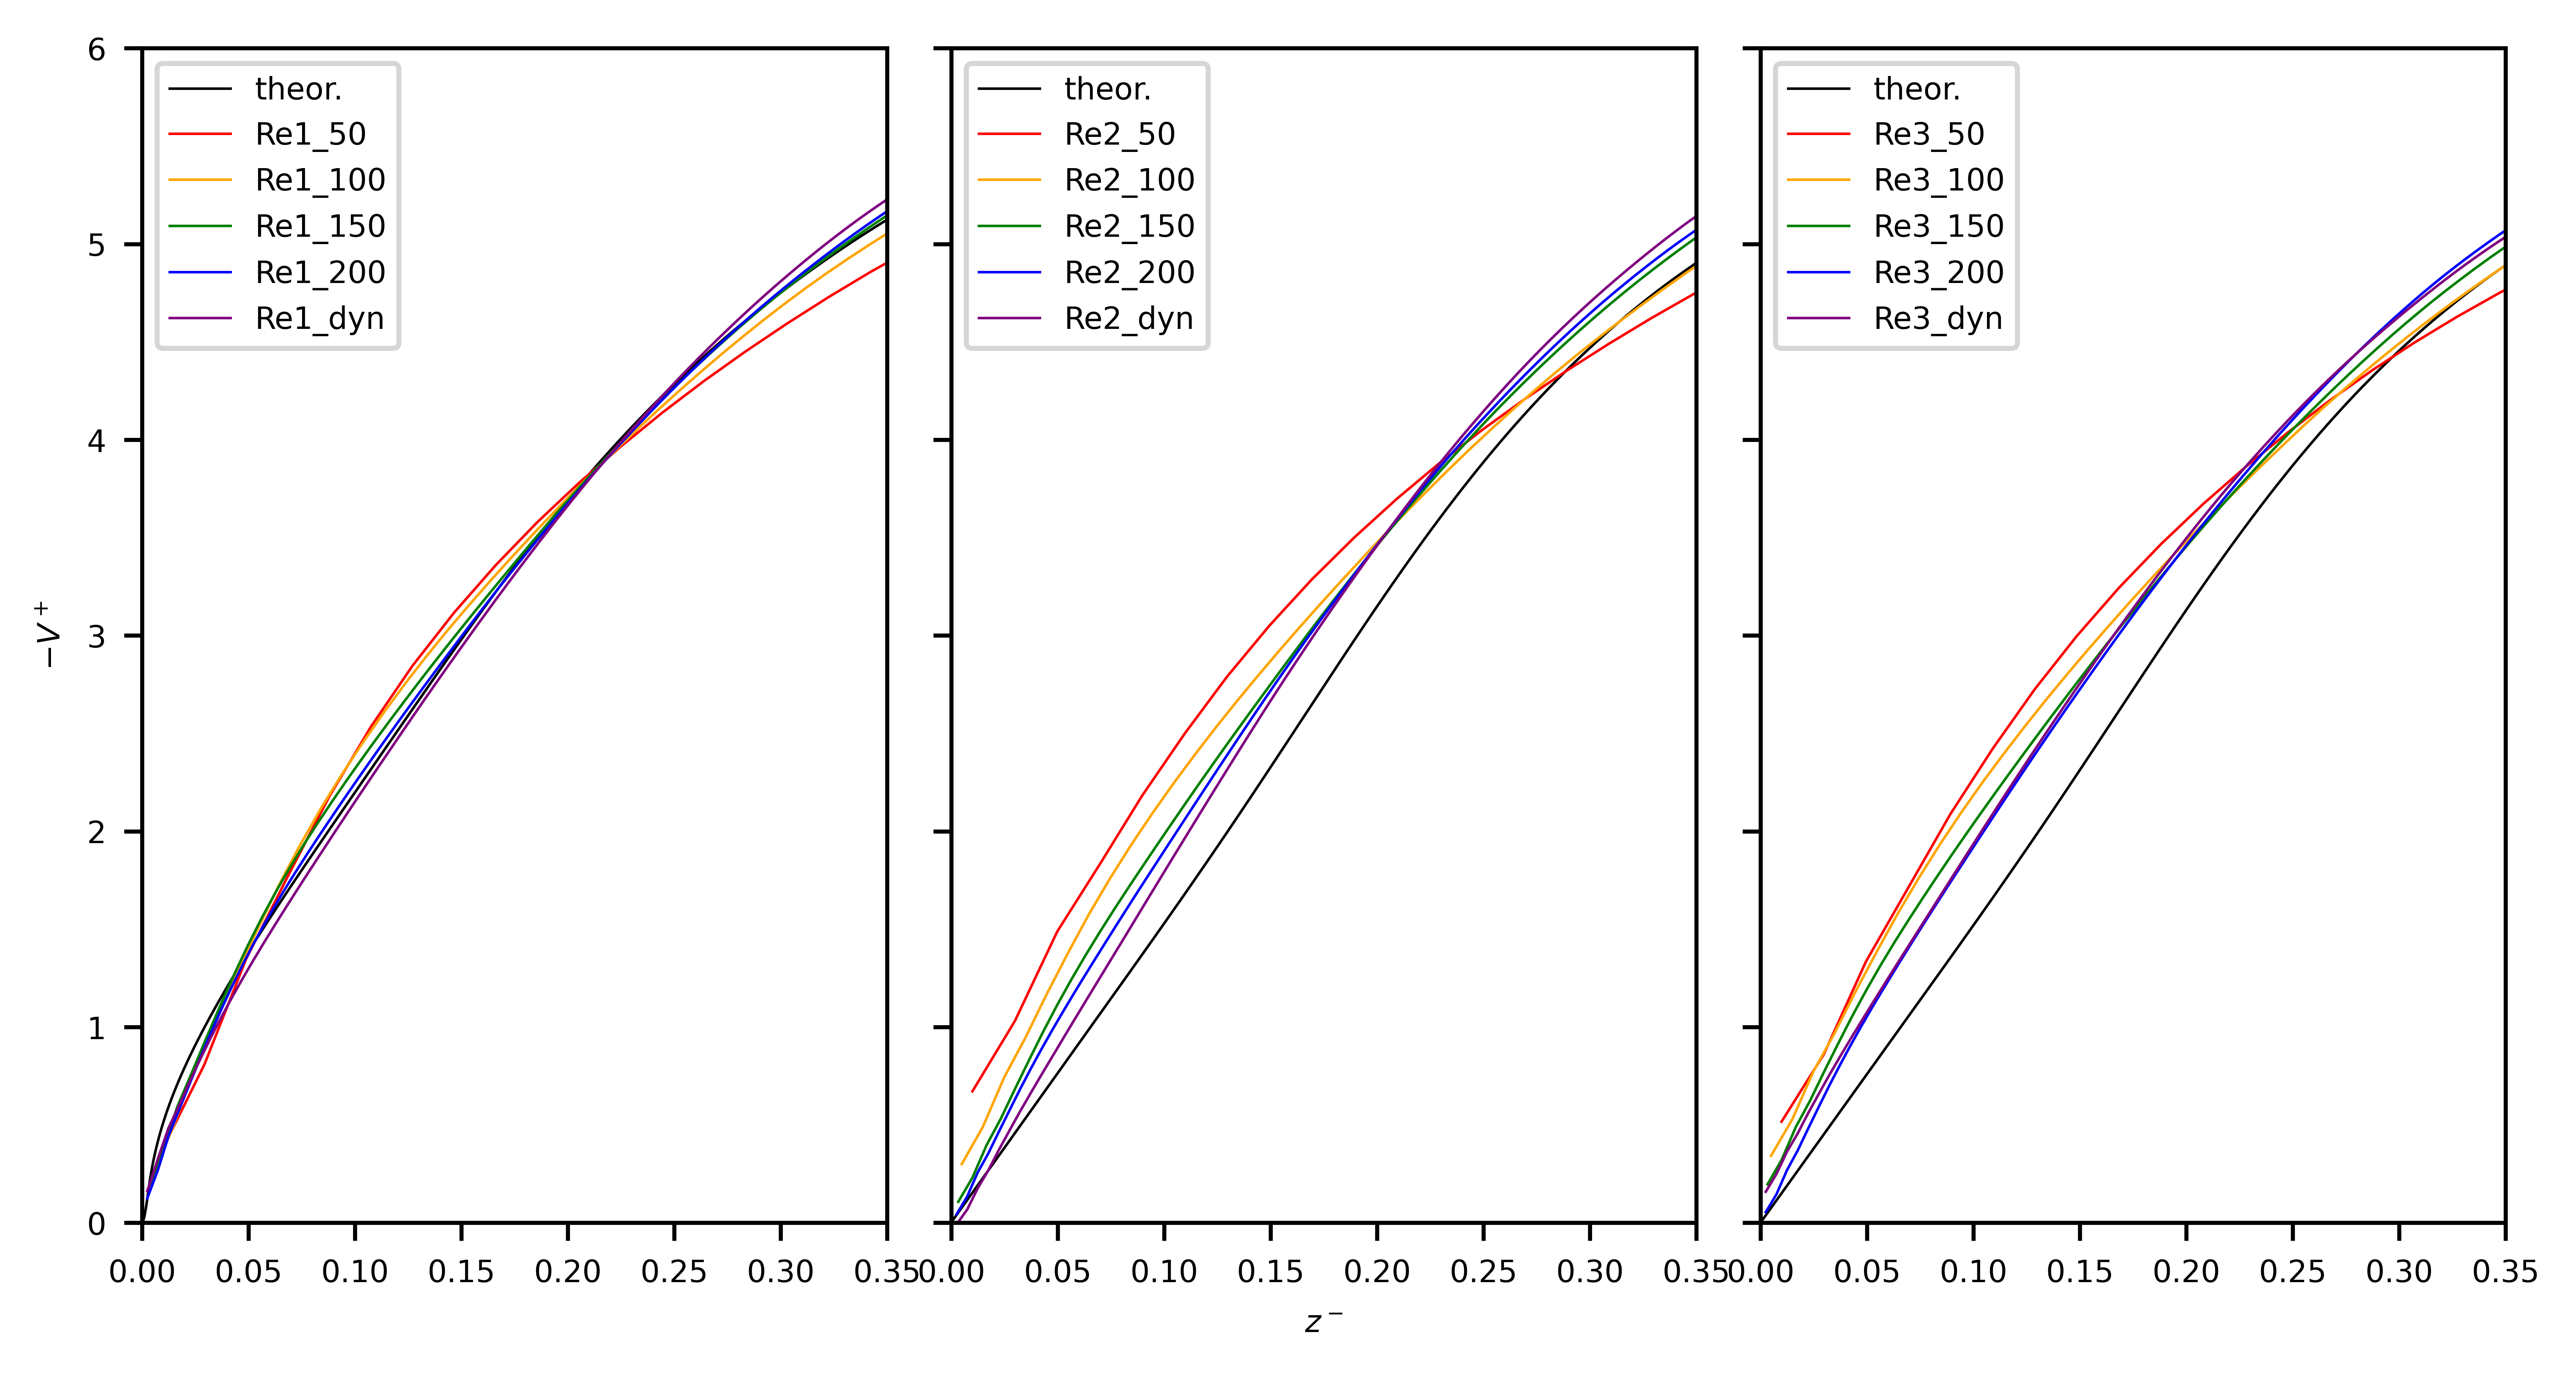
\includegraphics[width=\textwidth]{figures_2024/d3y_3Re_v_outer_lin.png}
%DIFDELCMD < }
%DIFDELCMD <   %%%
\DIFdelendFL \DIFaddbeginFL \centerline{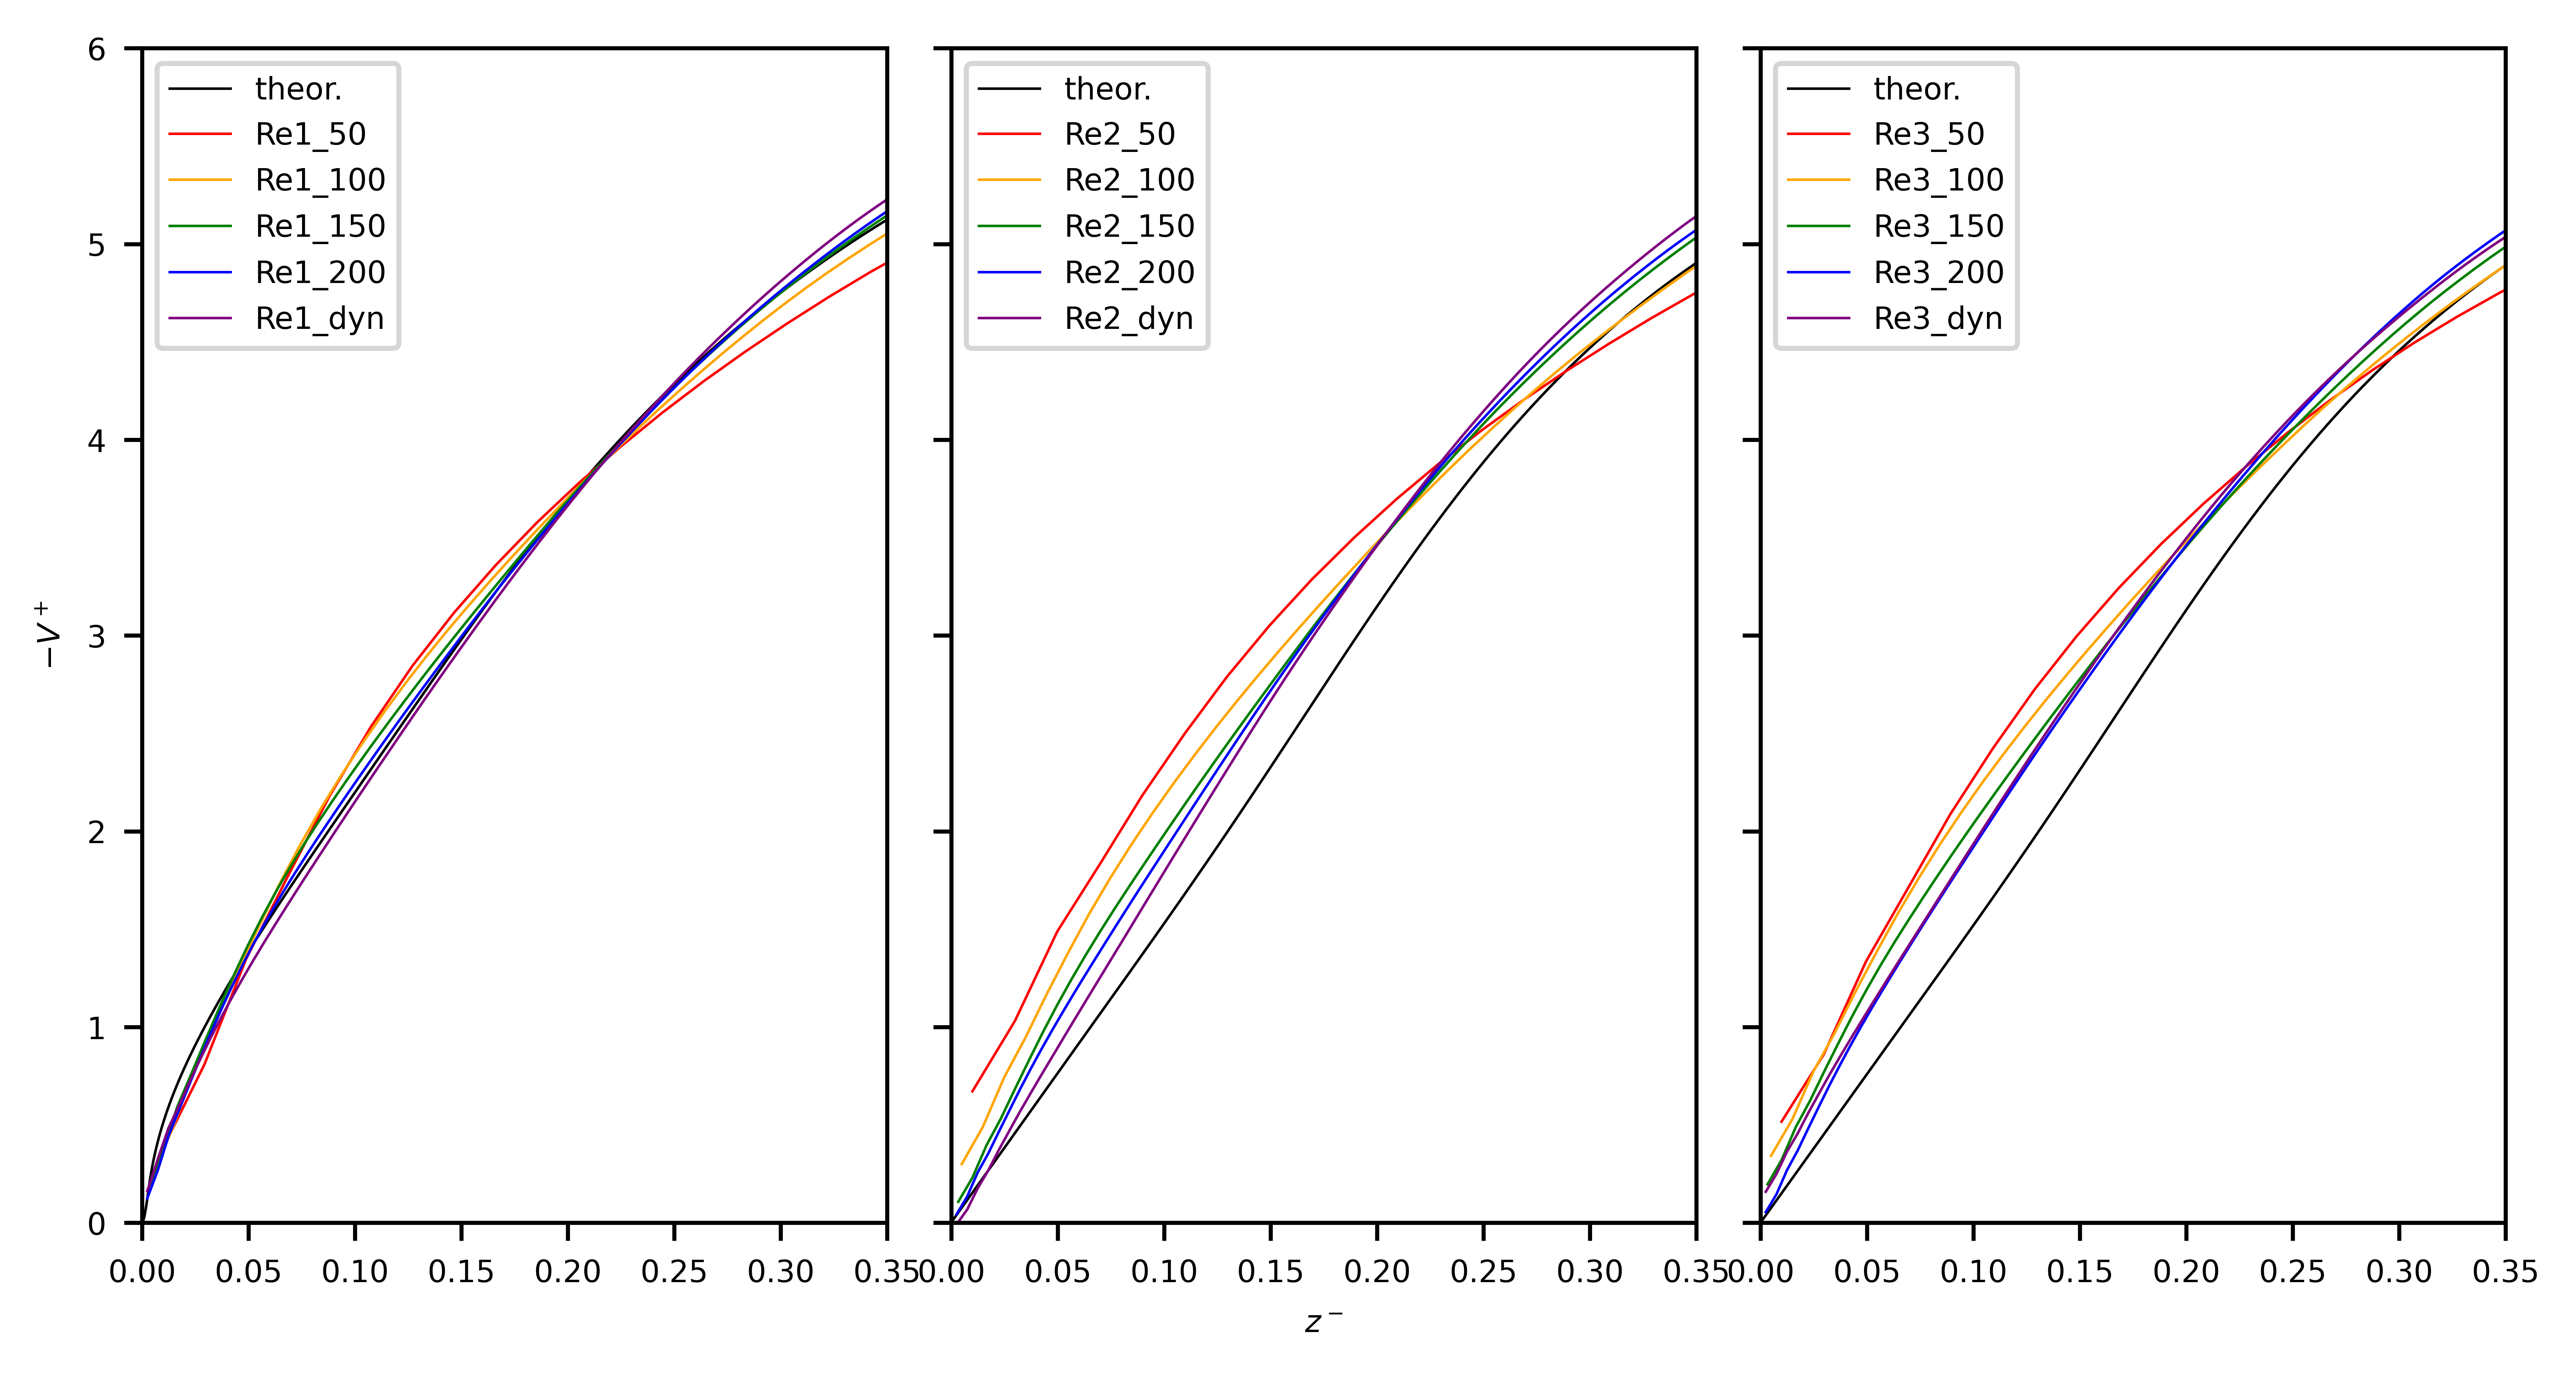
\includegraphics[width=\textwidth]{figures_2024/d3y_3Re_v_outer_lin.png}}
  \DIFaddendFL \caption{Span-wise velocity component in outer scaling}
  \DIFdelbeginFL %DIFDELCMD < \label{3Re_v_lin}
%DIFDELCMD < %%%
\DIFdelendFL \DIFaddbeginFL \label{fig:3Re_v_lin}
\DIFaddendFL \end{figure}

\DIFdelbegin \DIFdel{Figure \ref{3Re_v_lin} shows the }\DIFdelend \DIFaddbegin \DIFadd{he }\DIFaddend span-wise velocity component in the lower part of the boundary layer \DIFaddbegin \DIFadd{is shown in Fog.~\ref{fig:3Re_v_lin}}\DIFaddend . \todo{if we keep $V(z=\Delta)$ in the conclusion, add this here}. In the lowest part of $Re1$ ($z^-\lessapprox 0.05$), a part of the viscous layer is visible, where the velocity is slightly underestimated by the the LES. Above, the simulations \DIFdelbegin \DIFdel{$Re1\_200$ and $Re1\_dyn$ }\DIFdelend \DIFaddbegin \DIFadd{Re1\_200 and Re1\_dyn }\DIFaddend are very close to the theoretical curve. Lower resolution leads to an overestimation of the velocity in the logarithmic layer, which is consistent with a lack of large eddies \DIFdelbegin \DIFdel{that translates in a lack of mixing and thus a reduced turbulence level }\DIFdelend \DIFaddbegin \DIFadd{and thus too little mixing, reduced turbulence intensity }\DIFaddend and increased velocity gradients. Around $z^-=0.25$, while blending into the Ekman layer, the curves cross each other and \DIFaddbegin \DIFadd{aloft }\DIFaddend the coarse simulations \DIFdelbegin \DIFdel{begin to }\DIFdelend underestimate the velocity. For the higher $Re$ all simulations overestimate the velocity in the logarithmic layer \DIFdelbegin \DIFdel{, while coarser resolution leads to a higher velocity and finer resolution leads to a }\DIFdelend \DIFaddbegin \DIFadd{while finer resolution loeads to }\DIFaddend lower velocity and better agreement with the theoretical curve. Again, we see a crossing of the curves, between $z^-=0.2$ and $z^-=0.25$. A possible explanation of the fast increase and the steeper course of the coarser simulations is that the layers are coupled via less cells.

\subsection{Ekman layer}

Above the logarithmic layer, the Ekman layer follows, characterized by a change of wind direction. The course of the wind velocity vector is visualized by hodographs, as plotted in Fig. \ref{3Re_hodograph}. The hodograph of Re1\_X is followed quite closely by all resolutions. Hence, all simulations of the low-$\RE$ case---even Re1\_50---are resolved sufficiently to closely capture the course of the wind vector in the Ekman layer. The higher $\RE$ behave differently in the sense that the hodographs lie inside of the theoretical hodograph. An increased resolution ensures that at least the lowest grid point approaches the hodograph while the course of the hodograph's upper right part still does not reach the theoretical curve. 

\DIFaddbegin \DIFadd{\todo{translational statement to hodograph missing} }\DIFaddend In Fig. \ref{3Re_hodograph}, the cross indicates the lowest grid point and the plus indicates the height where the velocity for the boundary condition is taken from. To avoid taking a velocity from the first layer of the simulation, where the turbulent flow is poorly resolved, we took the horizontal velocity near $z^-=0.1$, where the mean velocity already veered away from the direction of the surface stress by around one third of $\alpha$. However, the veering does not seem to influence the resulting bulk stress $u_\star$ at the bottom: all but the coarsest resolutions yield a $u_\star$ very close to the theoretic reference.

\begin{figure}[ht]
  \centerline{
	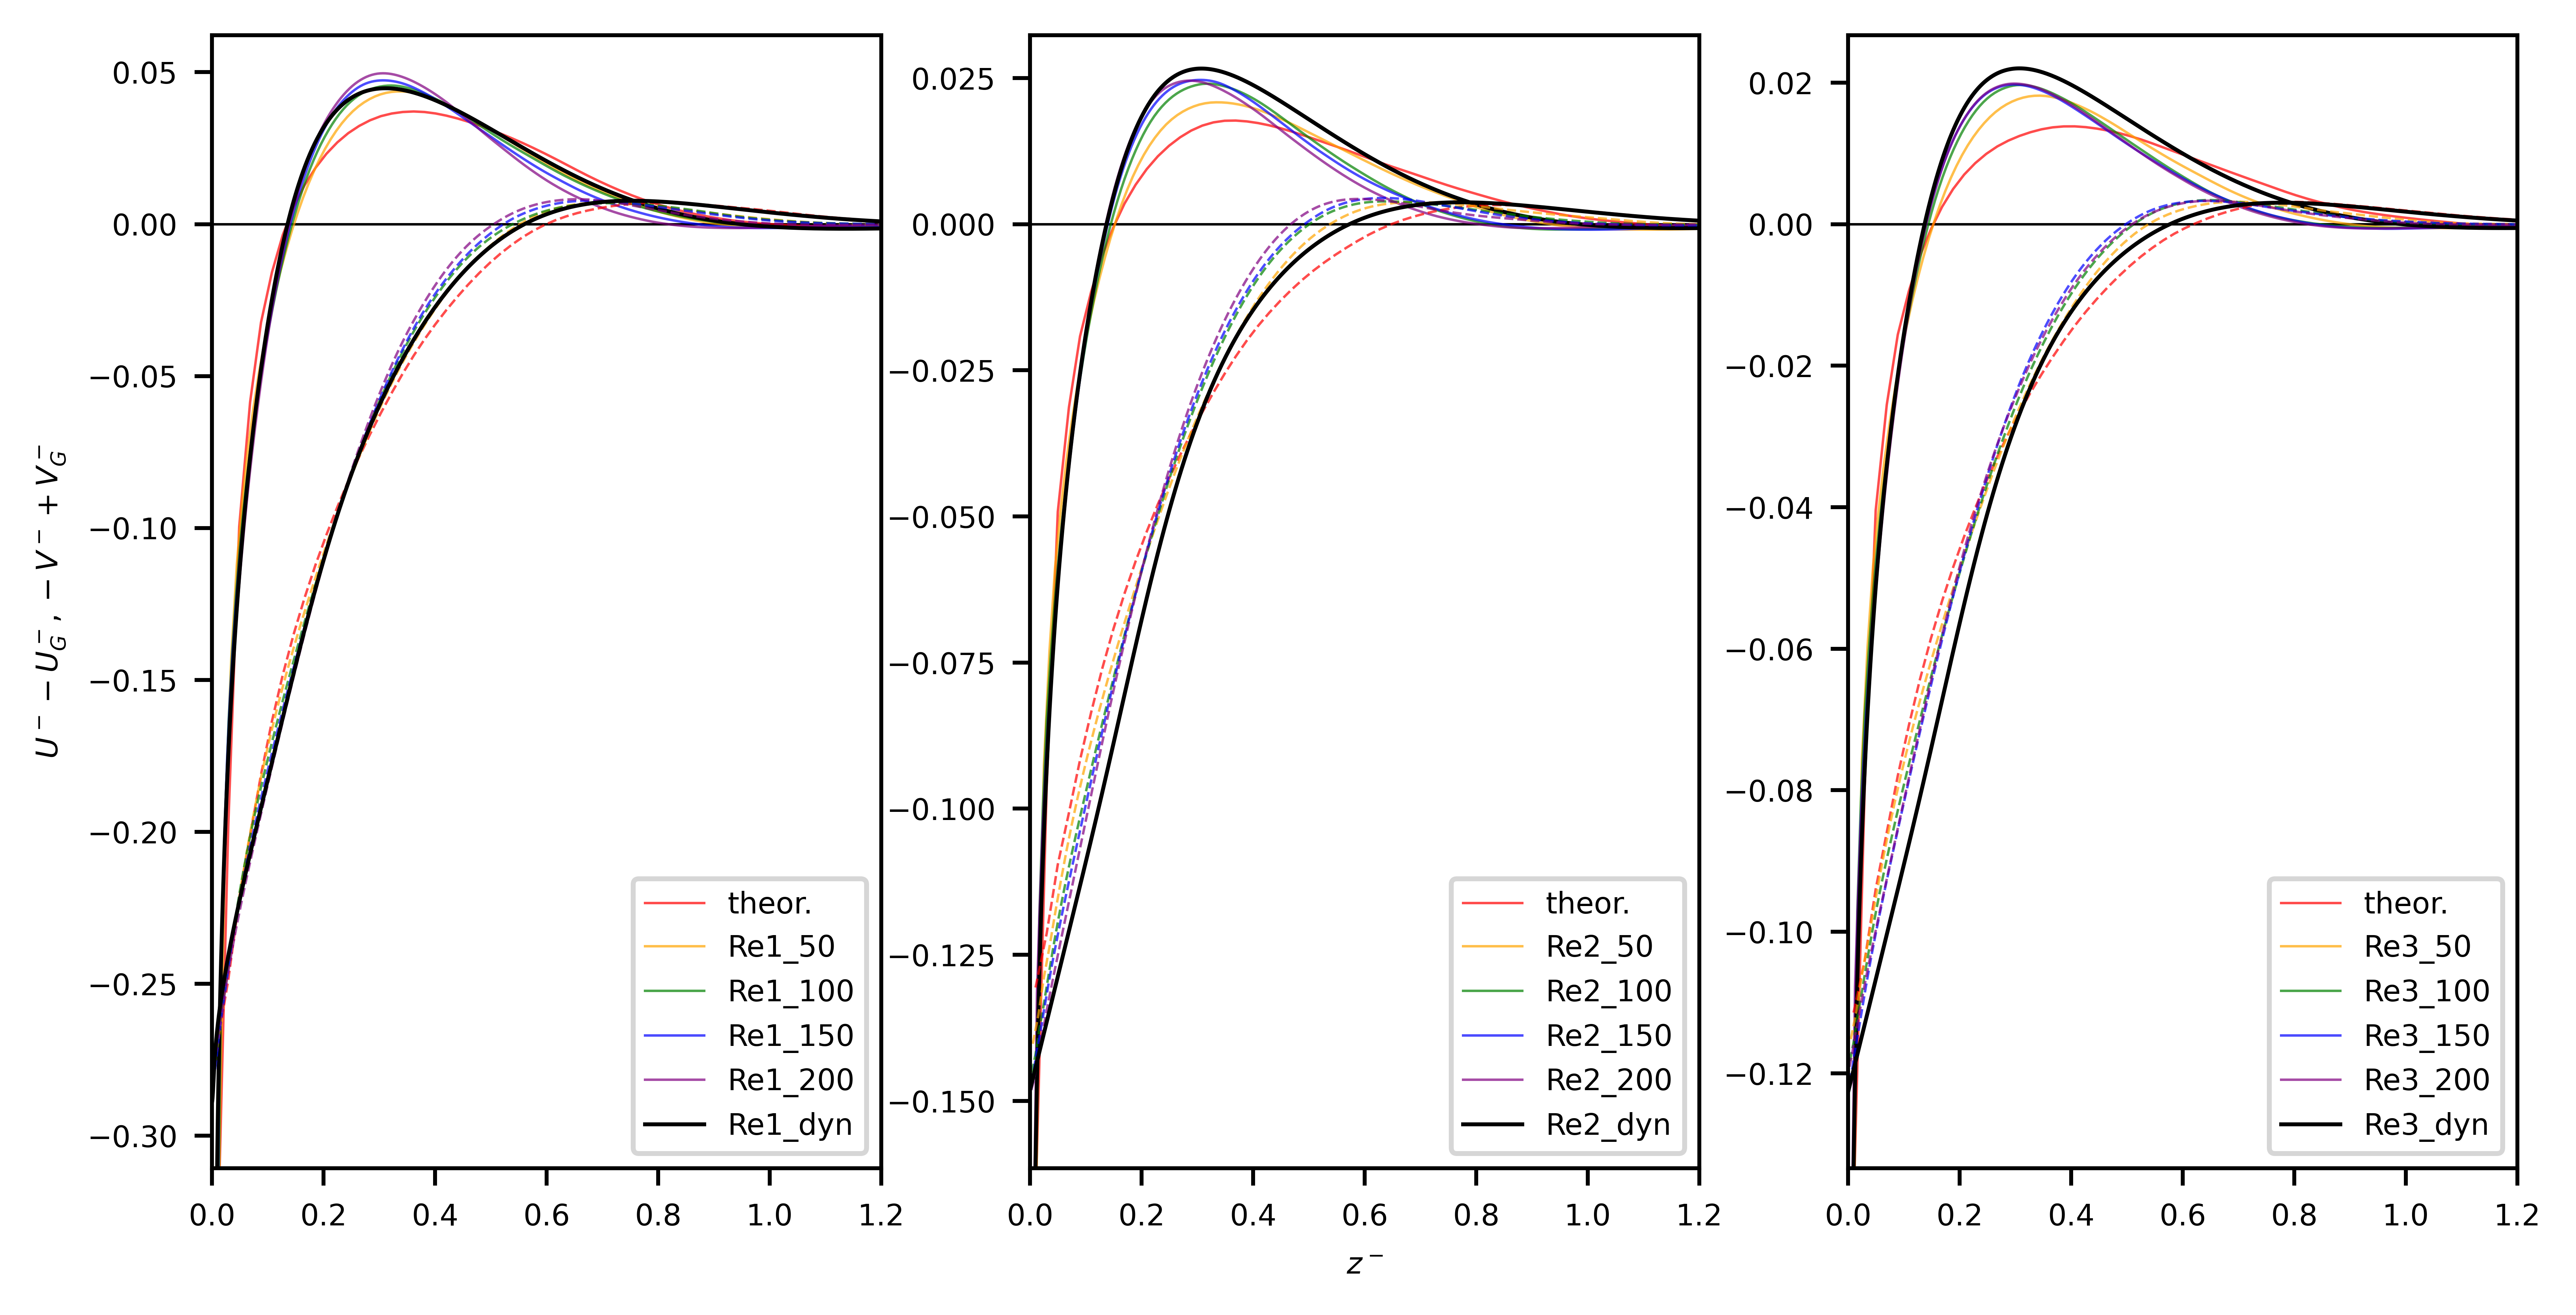
\includegraphics[width=\textwidth]{figures_2024/d3y_3Re_Ekman_lin.png}
}
  \caption{Shear-aligned velocity deficit in outer scaling. Solid lines: U-component, dashed lines: V-component}
  \DIFdelbeginFL %DIFDELCMD < \label{3Re_Ekman}
%DIFDELCMD < %%%
\DIFdelendFL \DIFaddbeginFL \label{fig:3Re_Ekman}
\DIFaddendFL \end{figure}

\DIFdelbegin \DIFdel{Figure \ref{3Re_Ekman} shows the }\DIFdelend \DIFaddbegin \DIFadd{The }\DIFaddend shear-aligned velocity deficit $U^--U^-_G$ (v-component accordingly) \DIFdelbegin \DIFdel{of the whole boundary layer. The strongest deviations from the theoretical profiles can be seen }\DIFdelend \DIFaddbegin \DIFadd{agrres well with the expected DNS-based profiles. The largest deviations occur }\DIFaddend for the coarsest LES near the super-geostrophic maximum of the U-component. Finer resolution leads to \DIFdelbegin \DIFdel{a very good agreementwith the extent of the maximum, which }\DIFdelend \DIFaddbegin \DIFadd{excellent agreement, }\DIFaddend also holds for the higher $\RE$. The super-geostrophic maximum is a consequence of vertical redistribution of momentum across the ABL; less redistribution leads to a less pronounced maximum. At the same time, of course, one would expect an increased level of turbulence to cause a flatter hodograph. \DIFdelbegin \DIFdel{BUT}\DIFdelend \DIFaddbegin \DIFadd{But}\DIFaddend , the surface veering is set rather by the interplay of \DIFdelbegin \DIFdel{MOST }\DIFdelend \DIFaddbegin \DIFadd{surface-layer turbulence }\DIFaddend and the prescribed roughness while the profile in the Ekman layer is \DIFdelbegin \DIFdel{a resolvedquantity}\DIFdelend \DIFaddbegin \DIFadd{resolved}\DIFaddend . However, for higher Reynolds numbers $Re2$ and $Re3$, the maximum velocity in x-direction is still not reached by the LES and the approach of the geostrophic wind in the upper part of the boundary layer takes place at lower heights than in theory. This is even more obvious for the V-component, where the maximum value is at a significantly lower height than in the theoretical curve. In general, a finer resolution leads to a lower location of the maximum. The maximum at lower heights might also explain the too high velocities in the logarithmic layer for the higher $Re$. 


\section{Conclusions}
\label{conclusion}

We studied truly neutral Ekman boundary layers---absent of capping inversions, non-stationarity, and surface heterogeneity. For the first time, an LES of the Ekman layer is \emph{a posteriori} validated against a DNS for an identical configuration. Despite the common assumption that viscosity as a parameter drops out in LES as a consequence of the turbulence closure, we considered a range of scale separations (Reynolds numbers) and found that for an exact representation of the surface turning and wall friction as well as the wind-turning profile, viscous effects need consideration. We derive an analytical relation demonstrating that --- given fixed surface properties --- the specification of $z_0$ implicitly defines a viscosity. The LES suffer from the dilemma, that in Ekman flow, some aspects of crucial importance happen on relatively small scales, such as the rotation-surface interaction which is confined to the inner layer.

With the wind-profile formulation developed in Part 1 of this work, we have a reference based on first principles for intermediate-Re simulations, and a quasi-reference for the higher-Re simulations. While we acknowledge that both the LES and the wind-profile model suffer from assumptions for high Reynolds number, their quantitative agreement across a wide range of scale separations hints towards the consistency. In particular, we understand that the grid convergence of LES towards the theoretical profiles underpins the inviscid scaling hypotheses in the development of the theory underlying part 1 of this paper.

We simulated three different Reynolds numbers while having DNS results for the lowest $\RE$. For the low $\RE$, viscous forces have a significant contribution to the balance of forces on the grid scale of the LES, hence we adapted the LES code to consider the fluid's viscosity in addition to the modeled eddy-viscosity. We did not introduce a roughness length $z_0$ at the lower boundary as additional parameter but deduced $z_0$ according to the law of the wall and the shear velocity expected according to the semi-empirical law by \cite{spalart1989theoretical}. The interplay of geostrophic wind, shear velocity, and roughness length in the simulation showed remarkable consistency, which supports the value of the adapted boundary condition at the bottom \citep{maronga2017formulation}. The dependence of the LES solution on the grid cell size was investigated through a comparison of four different resolutions. The setups of all $\RE$ use similar grid sizes in terms of the outer scale ($\Delta^-=\Delta/\delta=const.$) but different grid sizes in terms of the inner scale ($\Delta^+=\delta^+\cdot const. = Re_\tau\cdot const.$). This means that from an inner scale perspective the high Reynolds numbers were much less well resolved.

The convergence towards the theoretical profile expressed itself in different major aspects of the flow. To reach the expected total rotation $\alpha_\star$, a sufficient resolution was necessary. Furthermore, a sufficient vertical resolution was needed to simulate a logarithmic layer with a constant K\'arm\'an measure in some vertical extent.

A resolution of 150 grid levels below $\delta$ resolves well the boundary layer across all $\RE$, in agreement with the findings of \cite{wurps2020grid}. Their study demonstrated successful resolution of the neutral simulation with more than 100 grid levels within the boundary layer $\delta_{95}$. The ratio $\delta_{95}/\delta$ is approximately $2/3$ (gradually decreasing with Reynolds number). Therefore, having 150 grid levels within $\delta$ roughly corresponds to around 100 grid levels within $\delta_{95}$.

In summary, we synthesize some technical recommendations for the correct simulation of Ekman layer dynamics on a process level:
\begin{itemize}
\item The roughness parameter ($z_0$) essentially defines a Reynolds number of the LES Problem
\item $V|_{z=\Delta} < u_\star$ for an accurate matching of the hodograph and proper quantification of $\alpha_\star$. \todo{where is this in the results?}
\item There should exist a logarithmic layer, or explicit consideration of viscous interaction with the surface; otherwise the assumptions of the surface closure (MOST / dynamic wall model) will fail.
\item The parameters $\alpha_\star$ and $u_\star$ characterizing the bulk Ekman dynamics (across the vertical extent of the boundary layer) are matched by the LES if---in a three-dimensionally isotropic grid---more than 150 grid points are used in the vertical direction.
\item For very high resolution or relatively small Reynolds number, the viscous friction needs to be taken into account as the modeled eddy viscosity may locally drop to zero.
\end{itemize}

When these considerations are taken into account, LES becomes possible at uncommonly low Reynolds number and resolution, which allows a quantitative comparison to state-of-the art DNS.

Some resolution and best-practice constraints developed in this work are strong, in some cases even prohibitive. They result from the externality of the flow, i.e. the presence of non-turbulent fluid aloft which leads to a duality of scales (cf. section \ref{universal_profile}): both the inner and outer dynamics need to be visible to the resolved LES scales, at least to some extent. Despite these relatively strong constraints, we appreciate the capability of LES which, for example in case Re3, can appropriately match both $u_\star$, $\alpha_\star$ and the hodograph with the first grid point located at about $10^6$ wall units. This means, there is a gap in resolution in comparison to a true DNS of five to six orders of magnitude per direction; illustrating that a DNS at this scale would be prohibitive and will remain so for a foreseeable time. From this inner, or small-scale perspective, a requirement of few hundred grid points across the boundary layers is not a lot.

We did not see a second logarithmic layer as \cite{jiang2018large} neither in the theoretical formulation nor in our simulations. A reason might be their introduction of the additional parameter $z_0$. \todo{keep this paragraph? After our discussion about the change of Re when introducing a roughness length I don't believe this explanation anymore...}

The theoretical formulation of mean velocity profiles within the turbulent Ekman layer can serve as \DIFdelbegin \DIFdel{comprehensive }\DIFdelend benchmark for model frameworks such as LES. These reference profiles offer a deeper analysis beyond the conventional assessment of the logarithmic increase in wind speed within the Prandtl layer. Comparing simulation results to the expected bulk parameters $u_\star$ and $\alpha_\star$ and to the hodograph and conducting a detailed evaluation of the wind speed profiles can yield valuable insights into the correct interplay among the model's grid resolution, turbulence closure, and boundary conditions. In the future, expanding the theoretical profiles to include additional aspects, such as temperature stratification, could potentially provide an even more valuable reference.

\section{Acknowledgements}

The simulations were performed at the HPC Cluster EDDY, located at the University of Oldenburg (Germany) and funded by the Federal Ministry for Economic Affairs and Energy (Bundesministeriums für Wirtschaft und Energie) under grant number 0324005.

\bibliographystyle{plainnat}
\DIFdelbegin %DIFDELCMD < \bibliography{papers.bib}
%DIFDELCMD < %%%
\DIFdelend \DIFaddbegin \bibliography{papers.bib,ansorge.bib}
\DIFaddend 

\end{document}

